\chapter{Dataset local}
\label{capitulo5}
\lhead{Capítulo 5. \emph{Dataset local}}


\section{Introducción}
El objetivo de este capítulo es explicar la elaboración de un dataset visual inercial, a través de la construcción de un robot prototipo, la adquisición de datos de odometría de los encoders del robot, de la captura de imágenes de la cámara empleada, y de la adquisición de las medidas tomadas por la IMU.


\clearpage

\section{Descripción del prototipo}

El prototipo realizado consiste en un robot diferencial inicialmente diseñado para la categorría Sumo de la VII Competencia Nacional de Robótica CCSBOTS 2018. El prototipo tiene un peso de 2.9 kg y es capaz de soportar pesos de hasta 4kg. Posee una placa de control a bajo nivel de los motores del robot, y una Raspberry Pi 3 que es utilizada para controlar el robot utilizando un mando del tipo joystick a través de la interfaz bluetooth. El robot posee además encoders en sus ruedas que permiten tener datos de odometría. Este prototipo tiene una autonomía aproximada de 1 hora. La figura \ref{imagen:Robot} muestra la configuración final del robot. 

Más información puede ser encontrada en el \href{https://github.com/Robot-Sumo/}{\underline{repositorio de desarrollo del robot}} .


\begin{figure}[H]
	\centering		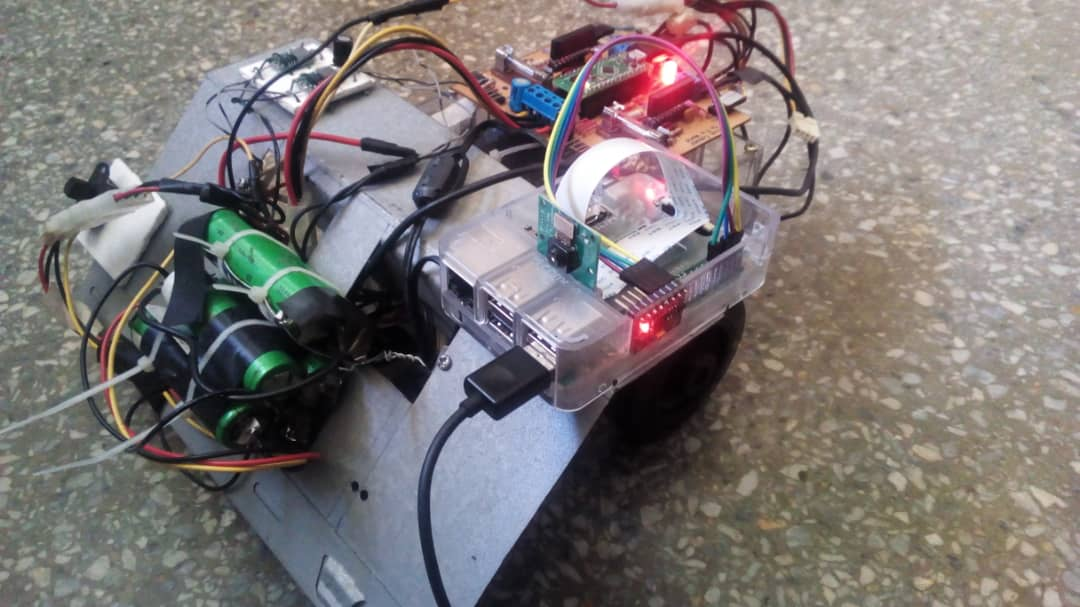
\includegraphics[width=0.7\linewidth]{imagenes/prototipo/Robot}
	\caption{Prototipo final.}
	\label{imagen:Robot}
\end{figure}


\section{Diseño mecánico}


El diseño mecánico del robot está centrado en el diseño de la caja de velocidad del robot. El modelaje 3D del robot se realizó utilizando Autocad como software de diseño y visualización del prototipo.



\subsection{Motores}

Los motores empleados en el diseño del robot fueron 4 motores con escobillas Mabuchi  C2162-60006. La figura \ref{imagen:prototipo/CajaMotores} presenta la configuración utilizada. El cuadro \ref{MabuchiDatasheet} presenta la información del motor suminastrada por el fabricante y el cuadro \ref{MabuchiResultados} presenta los resultados de las mediciones realizadas al motor para la caracterización de su resistencia de armadura.

\begin{figure}[H]
	\centering
	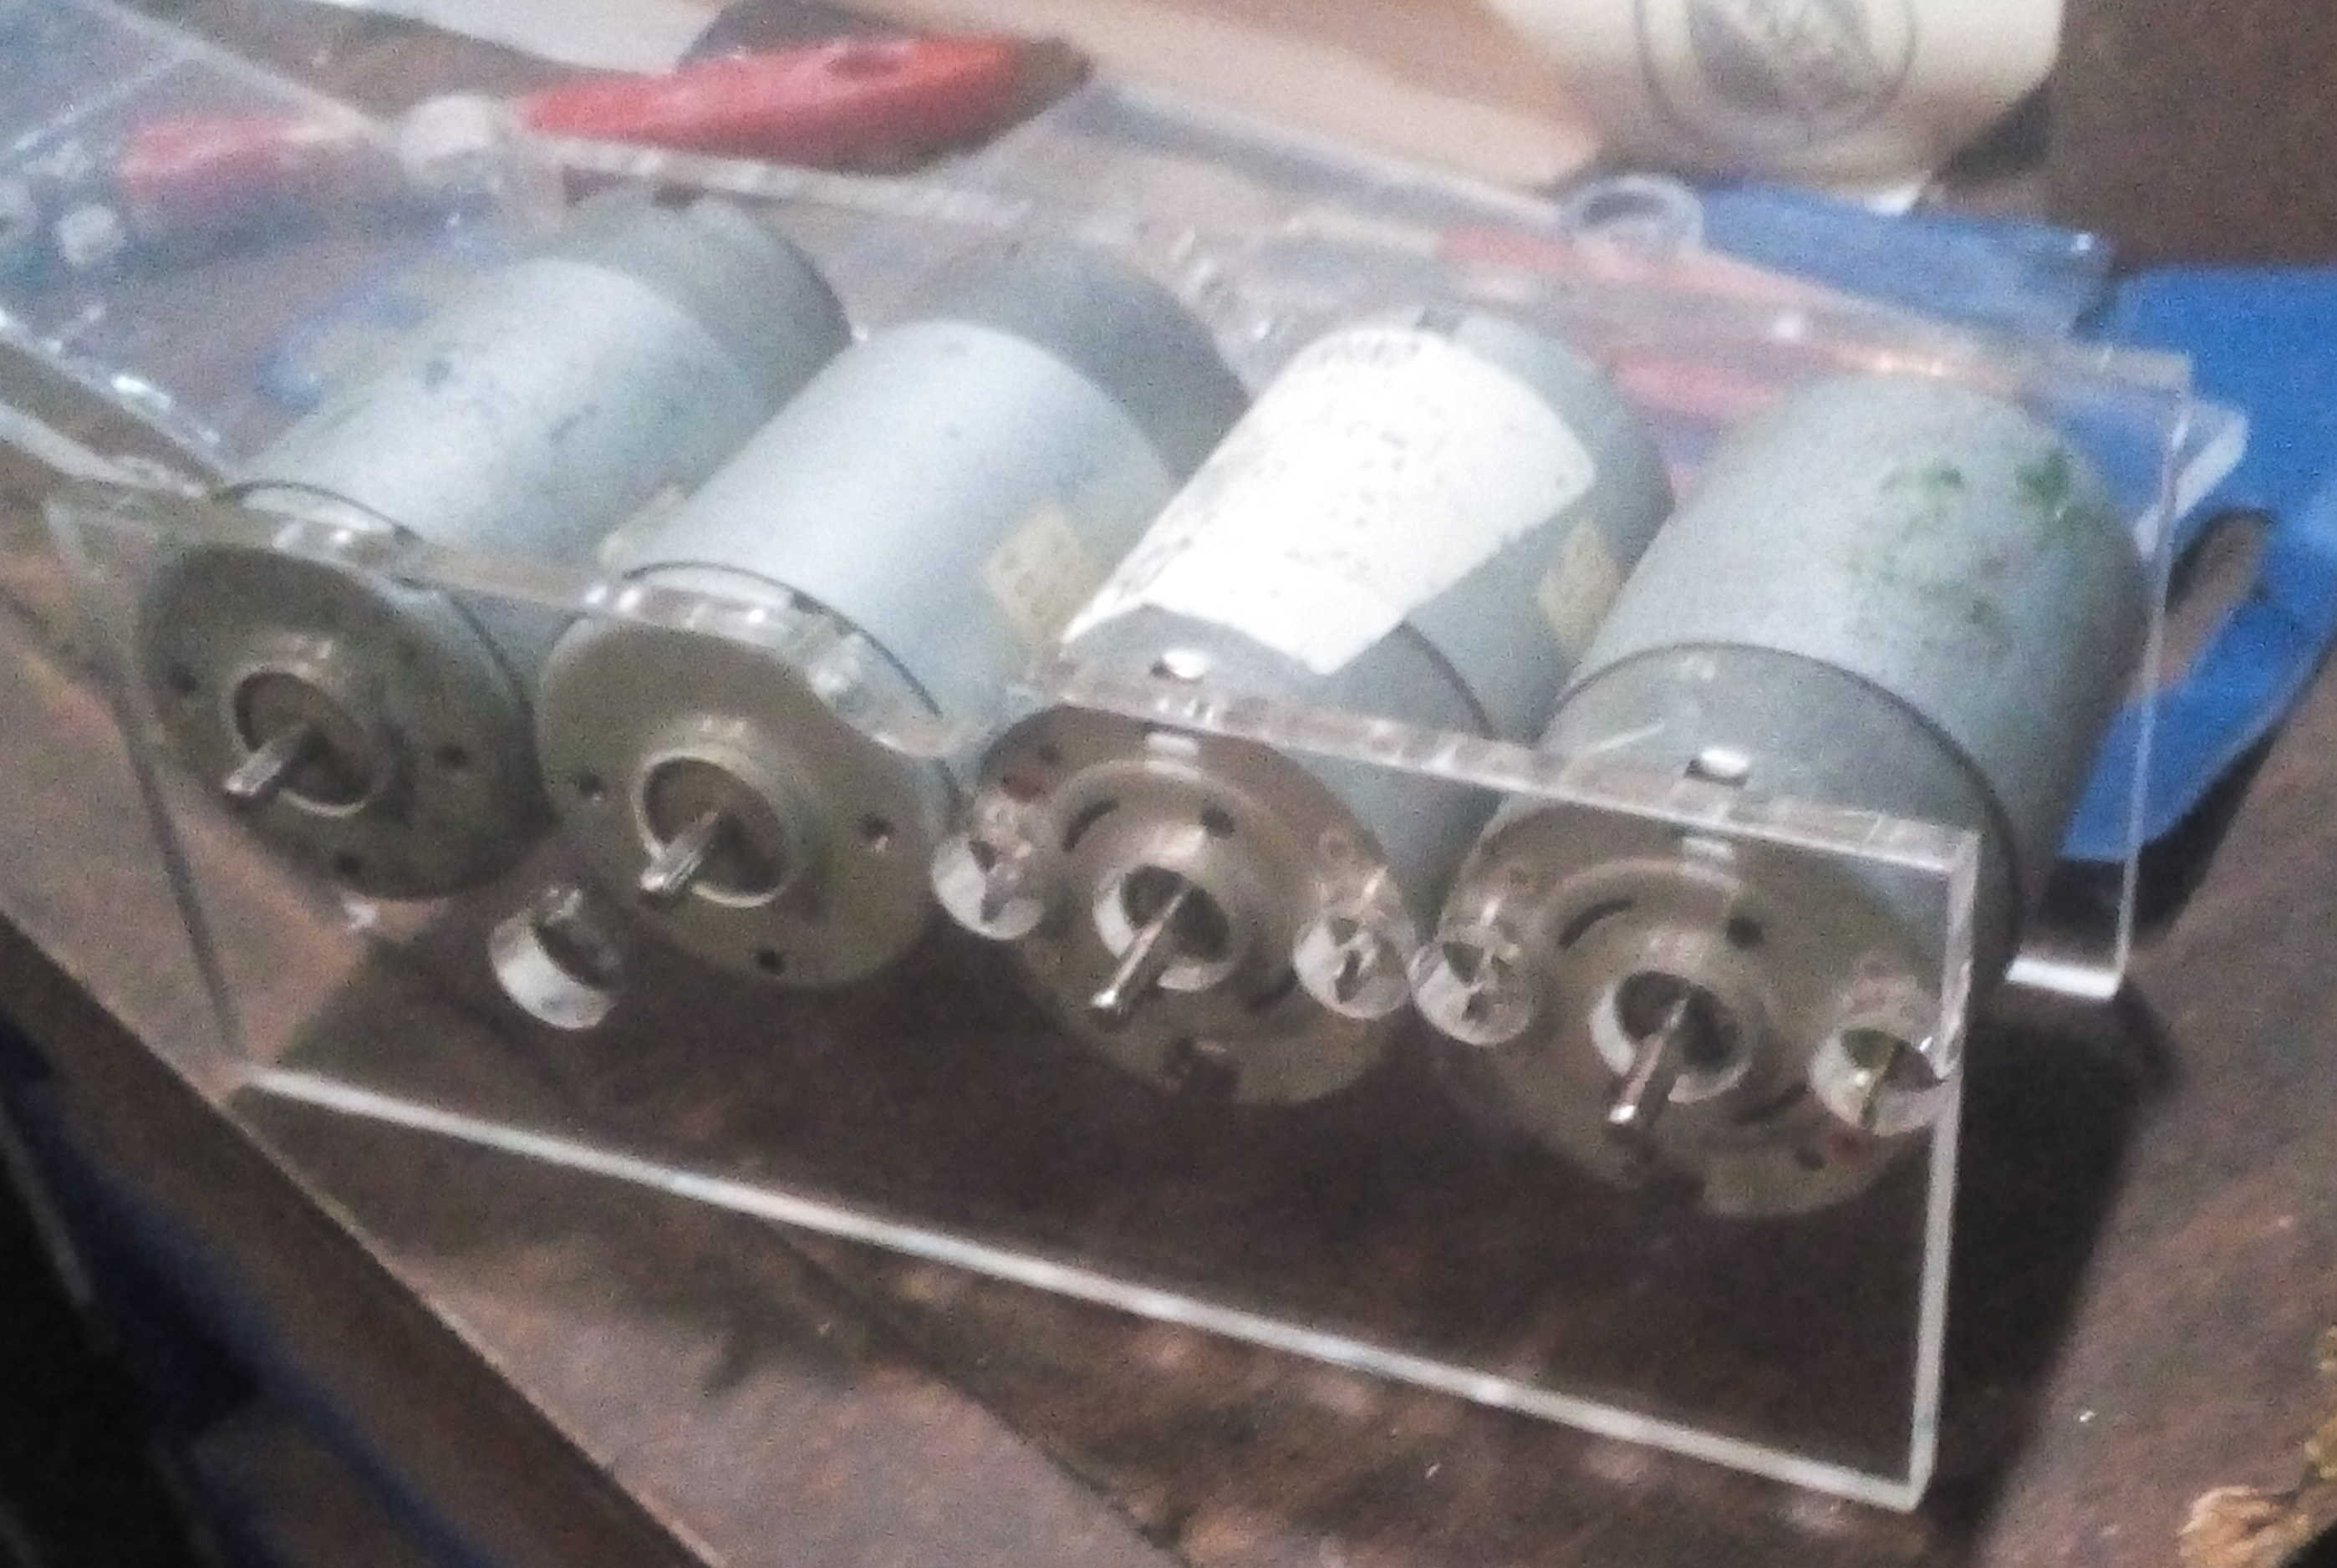
\includegraphics[width=0.7\textwidth]{prototipo/CajaMotores}
	\caption[Motores Mabuchi empleados en el diseño del prototipo]{Componentes de Hardware del robot.}
	\label{imagen:prototipo/CajaMotores}
\end{figure}

\begin{table}[htbp]
	\caption{Datos del motor Mabuchi proveidos por el fabricante.}
	\centering
	\begin{tabular}{|l|c|}
		\hline
		\multicolumn{ 2}{|c|}{\textbf{Motor  Mabuchi Brush C2162-60006 19-24v HP}} \\ \hline
		Rating [volts] & 19 \\ \hline
		Test [volts] & 24 \\ \hline
		Stall Torque [N-cm] & 28.7 \\ \hline
		Max. Power [Watts] & 34.2 \\ \hline
		Max. Power [mili-hp] & 45.8 \\ \hline
		Duration [sec] & 30 \\ \hline
		Energy [Joules] & 1026 \\ \hline
		Weight [grams] & 224 \\ \hline
		Power/Weight [Watts/kg] & 153 \\ \hline
		Energy/Weight [Joules/kg] & 4580 \\ \hline
	\end{tabular}
	\label{MabuchiDatasheet}
\end{table}



\begin{table}[htbp]
	\caption{Resultados de mediciones realizadas al motor.}
	\centering
	\begin{tabular}{|l|c|}
		\hline
		No Load Current [Amps] & 0.15 \\ \hline
		Resistance [Ohms] & 15 \\ \hline
		Stall Current [amps] & 1.6 \\ \hline
		No Load Speed [rpm] & 3500 \\ \hline
	\end{tabular}
	\label{MabuchiResultados}
\end{table}




Entre los datos relevantes en estos cuadros destacan la corriente del motor cuando es aplicado el máximo torque (Stall Current), la cual es utilizada para el diseño de las protecciones y de los puntos de referencia de los drivers, el máximo torque aplicado por el motor (Stall Torque)  y velocidad sin carga (No Load Speed), las cuales son utilizadas para el criterio de selección de la relación de reducción en el sistema de engranajes.

\subsection{Caja de velocidad}


El cuadro \ref{TablaPruebaEngranajes} presenta los resultados estimados  de torque máximo y velocidad máxima del robot para una relación de engranajes específica. En este caso la velocidad máxima del motor fue aproximada en 3000 rpm ya que la medición sin carga fue cercana a los 3500 rpm, y estas revoluciones bajan al presentar carga en el sistema de transferencia. El torque máximo inicial representa el aproximado de la suma del torque máximo de dos motores, cuyo valor se tomó cercano a 30 N-cm, respecto al valor de de 28.7 N-cm proveido por el fabricante en el cuadro \ref{MabuchiDatasheet}.

\begin{table}[htbp]
	\caption{Pruebas de diferentes relaciones de engranajes}
	\begin{tabular}{|l|r|r|r|r|}
		\hline
		\textbf{Relación final de engranajes} & \textbf{20} & \textbf{15} & \textbf{12} & \textbf{8} \\ \hline
		Velocidad máxima del motor (rpm) & 3000 & 3000 & 3000 & 3000 \\ \hline
		Radio de la rueda (cm) & 3.74 & 3.74 & 3.74 & 3.74 \\ \hline
		Velocidad máxima de la rueda (rpm) & 150 & 200 & 250 & 375 \\ \hline
		Velocidad máxima de la rueda (rev/s) & 15.708 & 20.944 & 26.18 & 39.27 \\ \hline
		Torque máximo del Motor (N-cm) & 60 & 60 & 60 & 60 \\ \hline
		\textbf{Torque máximo final (N-cm)} & \textbf{1200} & \textbf{900} & \textbf{720} & \textbf{480} \\ \hline
		\textbf{Velocidad máxima del robot (m/s)} & \textbf{0.59} & \textbf{0.78} & \textbf{0.98} & \textbf{1.47} \\ \hline
	\end{tabular}
	\label{TablaPruebaEngranajes}
\end{table}



Con los resultados obtenidos para diferentes relaciones de engranajes, se utilizó Unity para simular las propiedades dinámicas del robot y de esta manera seleccionar la relación de engranajes con la mejor relación torque-velocidad. En la figura \ref{imagen:prototipo/SimulacionUnity} se presenta una captura de esta simulación, en la cual el robot debía ser capaz de mover a un robot con un peso de 3kg con características similares.



\begin{figure}[H]
	\centering
	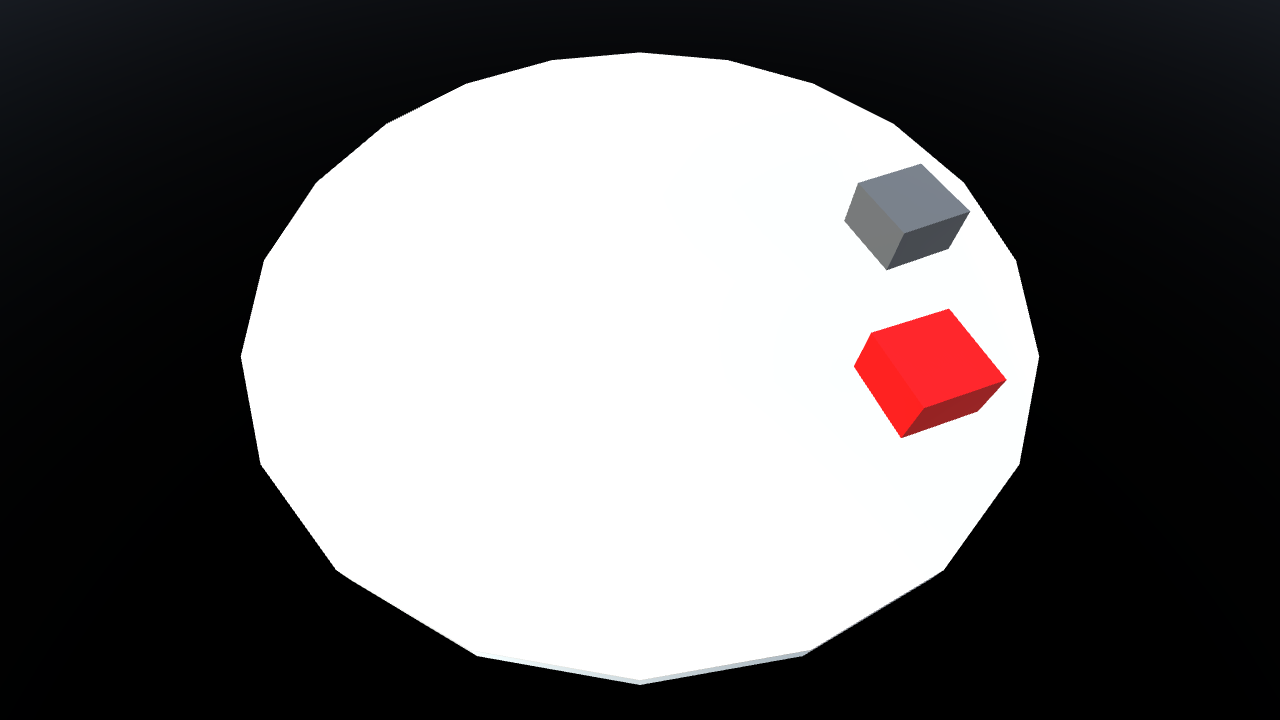
\includegraphics[width=0.7\textwidth]{imagenes/prototipo/SimulacionUnity}
	\caption{Simulación en Unity de las características dinámicas del robot para la elección de la relación de reducción de velocidad.}
	\label{imagen:prototipo/SimulacionUnity}
\end{figure}

La relación final de reducción seleccionada fue de  15:1. De esta forma, el sistema de engranajes fue diseñado para cumplir esta relación. La figura \ref{imagen:disenoEngranajesAutocad} presenta el diseño realizado. En éste, se tiene un engranaje de 20 dientes acoplado a un engranaje de 60 dientes, el cual se encuentra acoplado en su mismo eje a un engranaje de 20 dientes. Posterioremente se tiene un engranajes de transmision de 20 dientes que se encarga de transmitir la velocidad al engranaje de la rueda, el cual fue diseñado para tener 100 dientes. Este engranaje es el de mayor tamaño en la figura \ref{imagen:disenoEngranajesAutocad}. De esta forma se garantizó la relación de reducción a 15.

\begin{figure}[H]
	\centering
	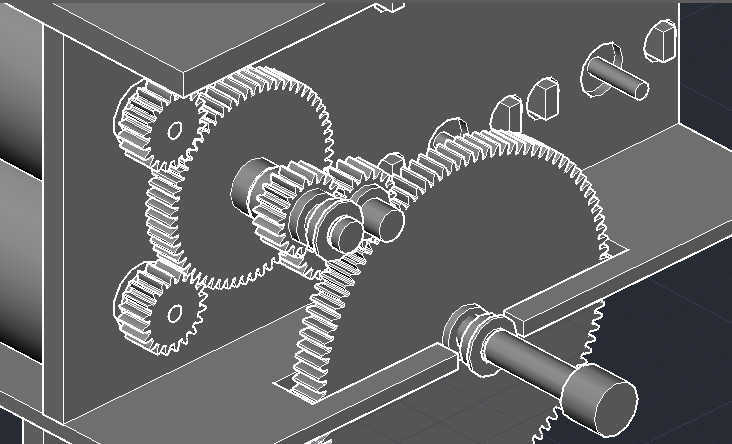
\includegraphics[width=0.7\linewidth]{imagenes/prototipo/EngranajesAutocad}
	\caption{Parte del modelado en 3D del robot realizado en Autocad}
	\label{imagen:disenoEngranajesAutocad}
\end{figure}


Las imágenes oresentadas en la figura \ref{imagen:construccionFinalRobot} presentan parte del proceso de construcción de la caja de velocidades. Los engranajes presentados fueron impresos utilizando el diseño 3D previamente realizado, y utilizando como material de impresión el polímero PLA. Cabe acotar que el empleo de dos motores por cada sistema de engranajes fue realizado para aumentar el torque de la caja de velocidad.

\begin{figure}[H]
	\centering		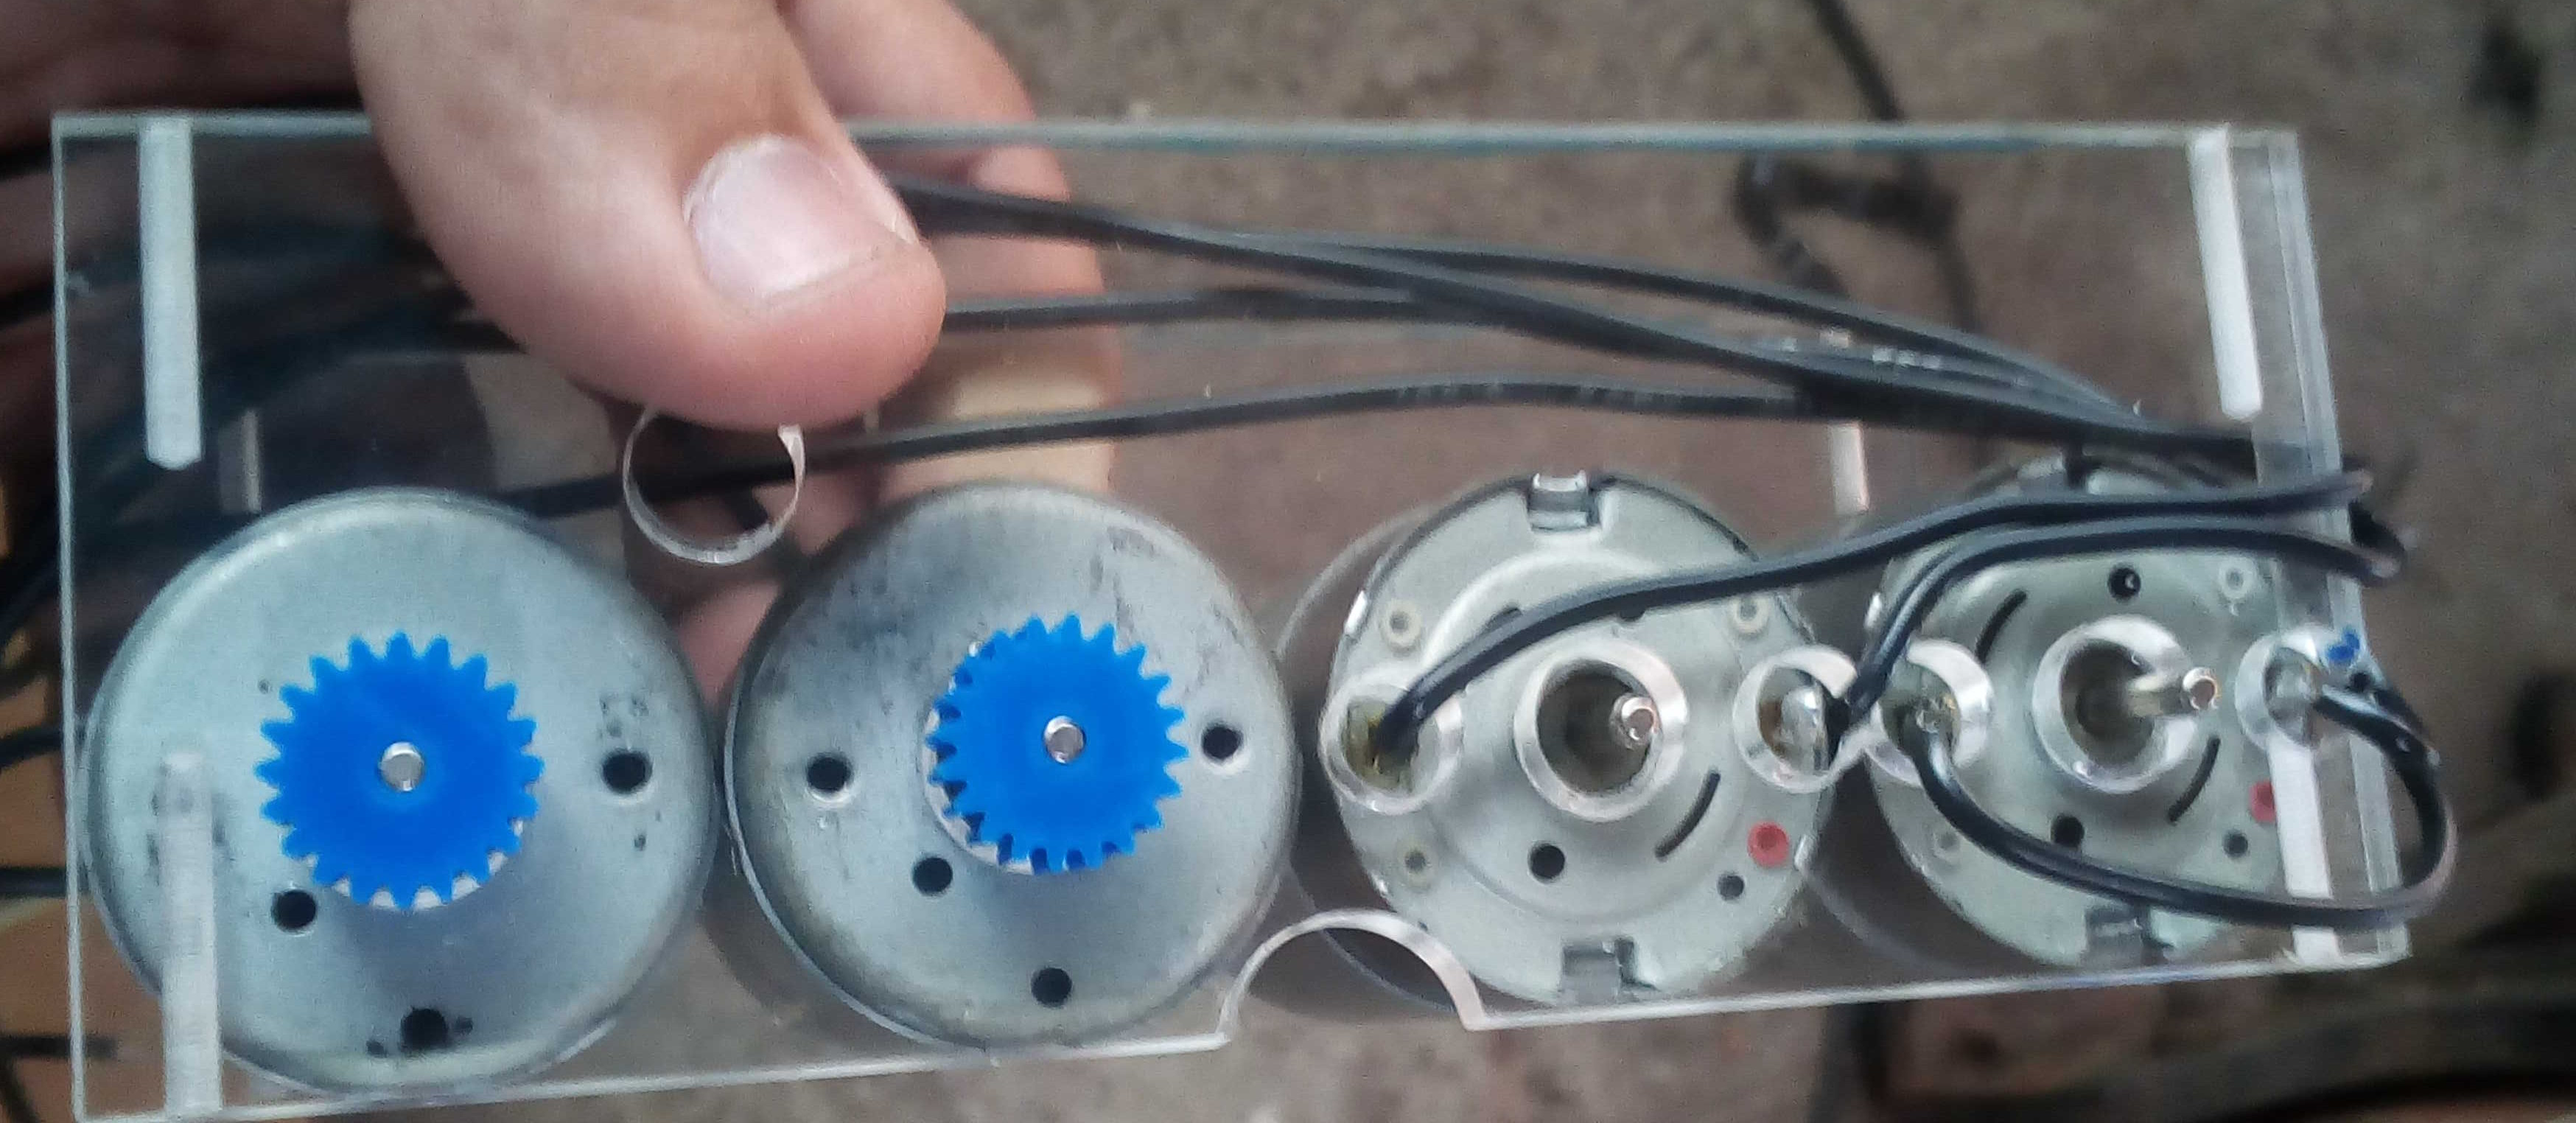
\includegraphics[width=0.7\linewidth]{imagenes/prototipo/Motores}
	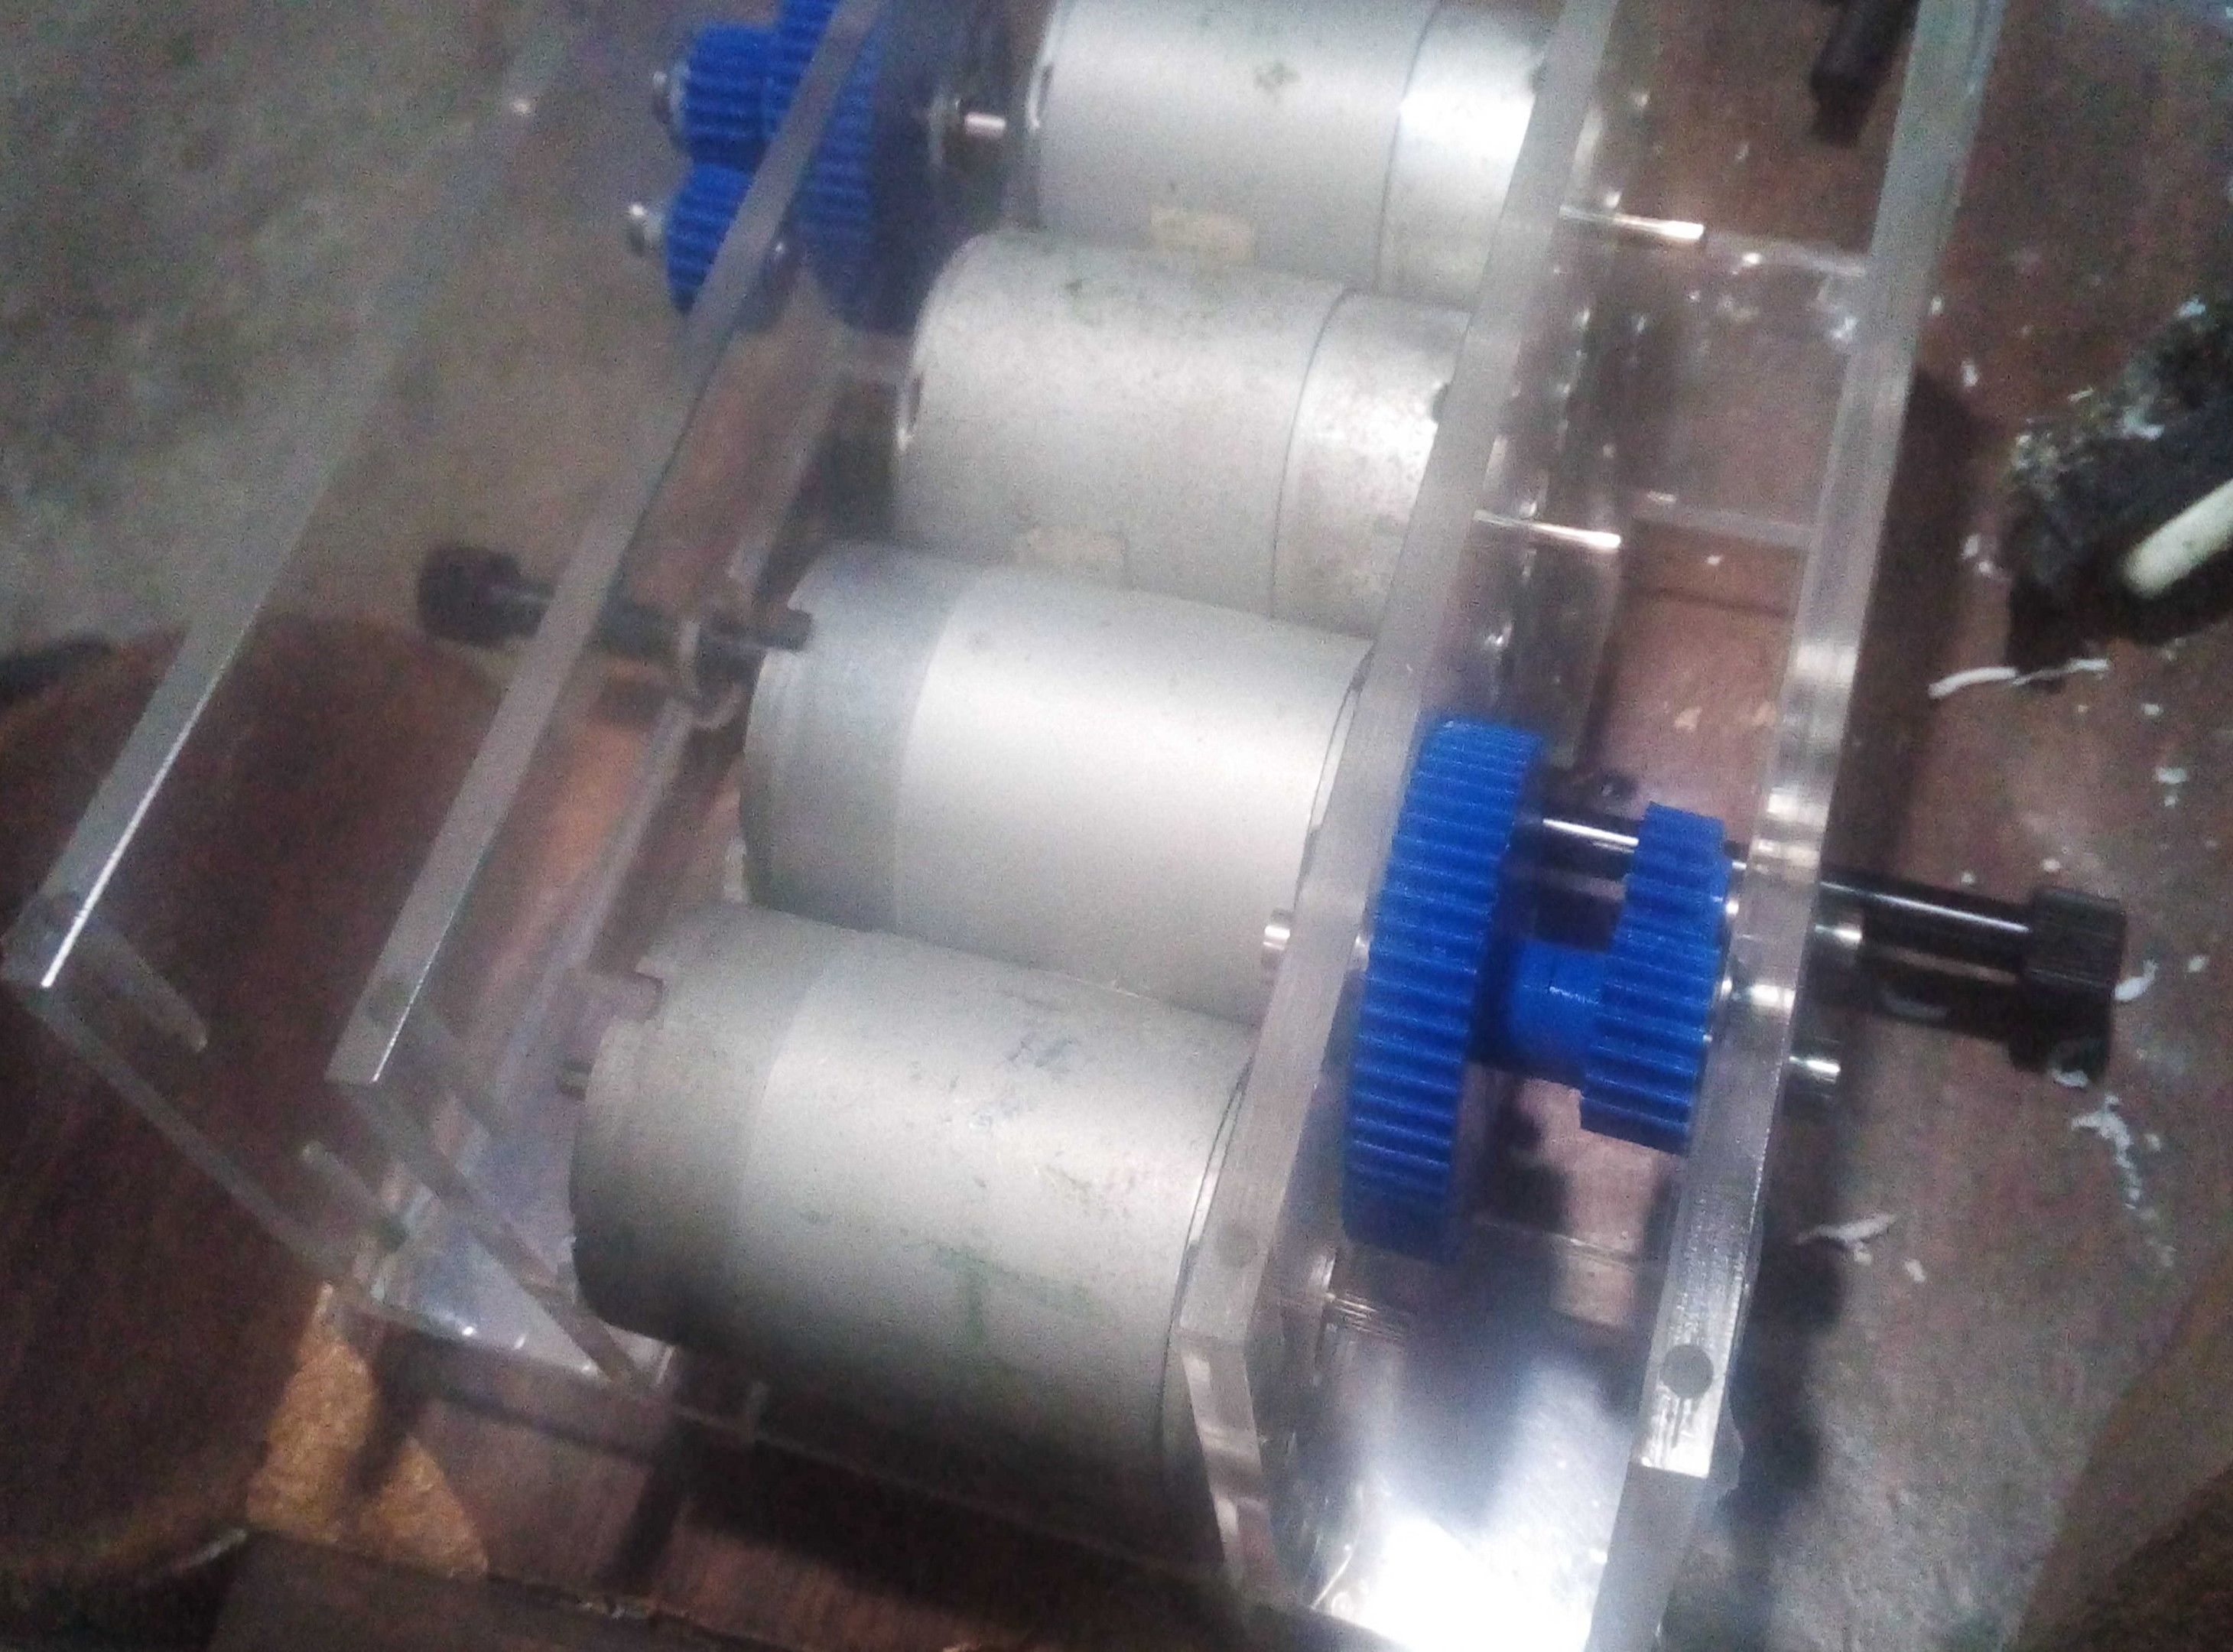
\includegraphics[width=0.4\linewidth]{imagenes/prototipo/CajaColocandoEngranejes}
	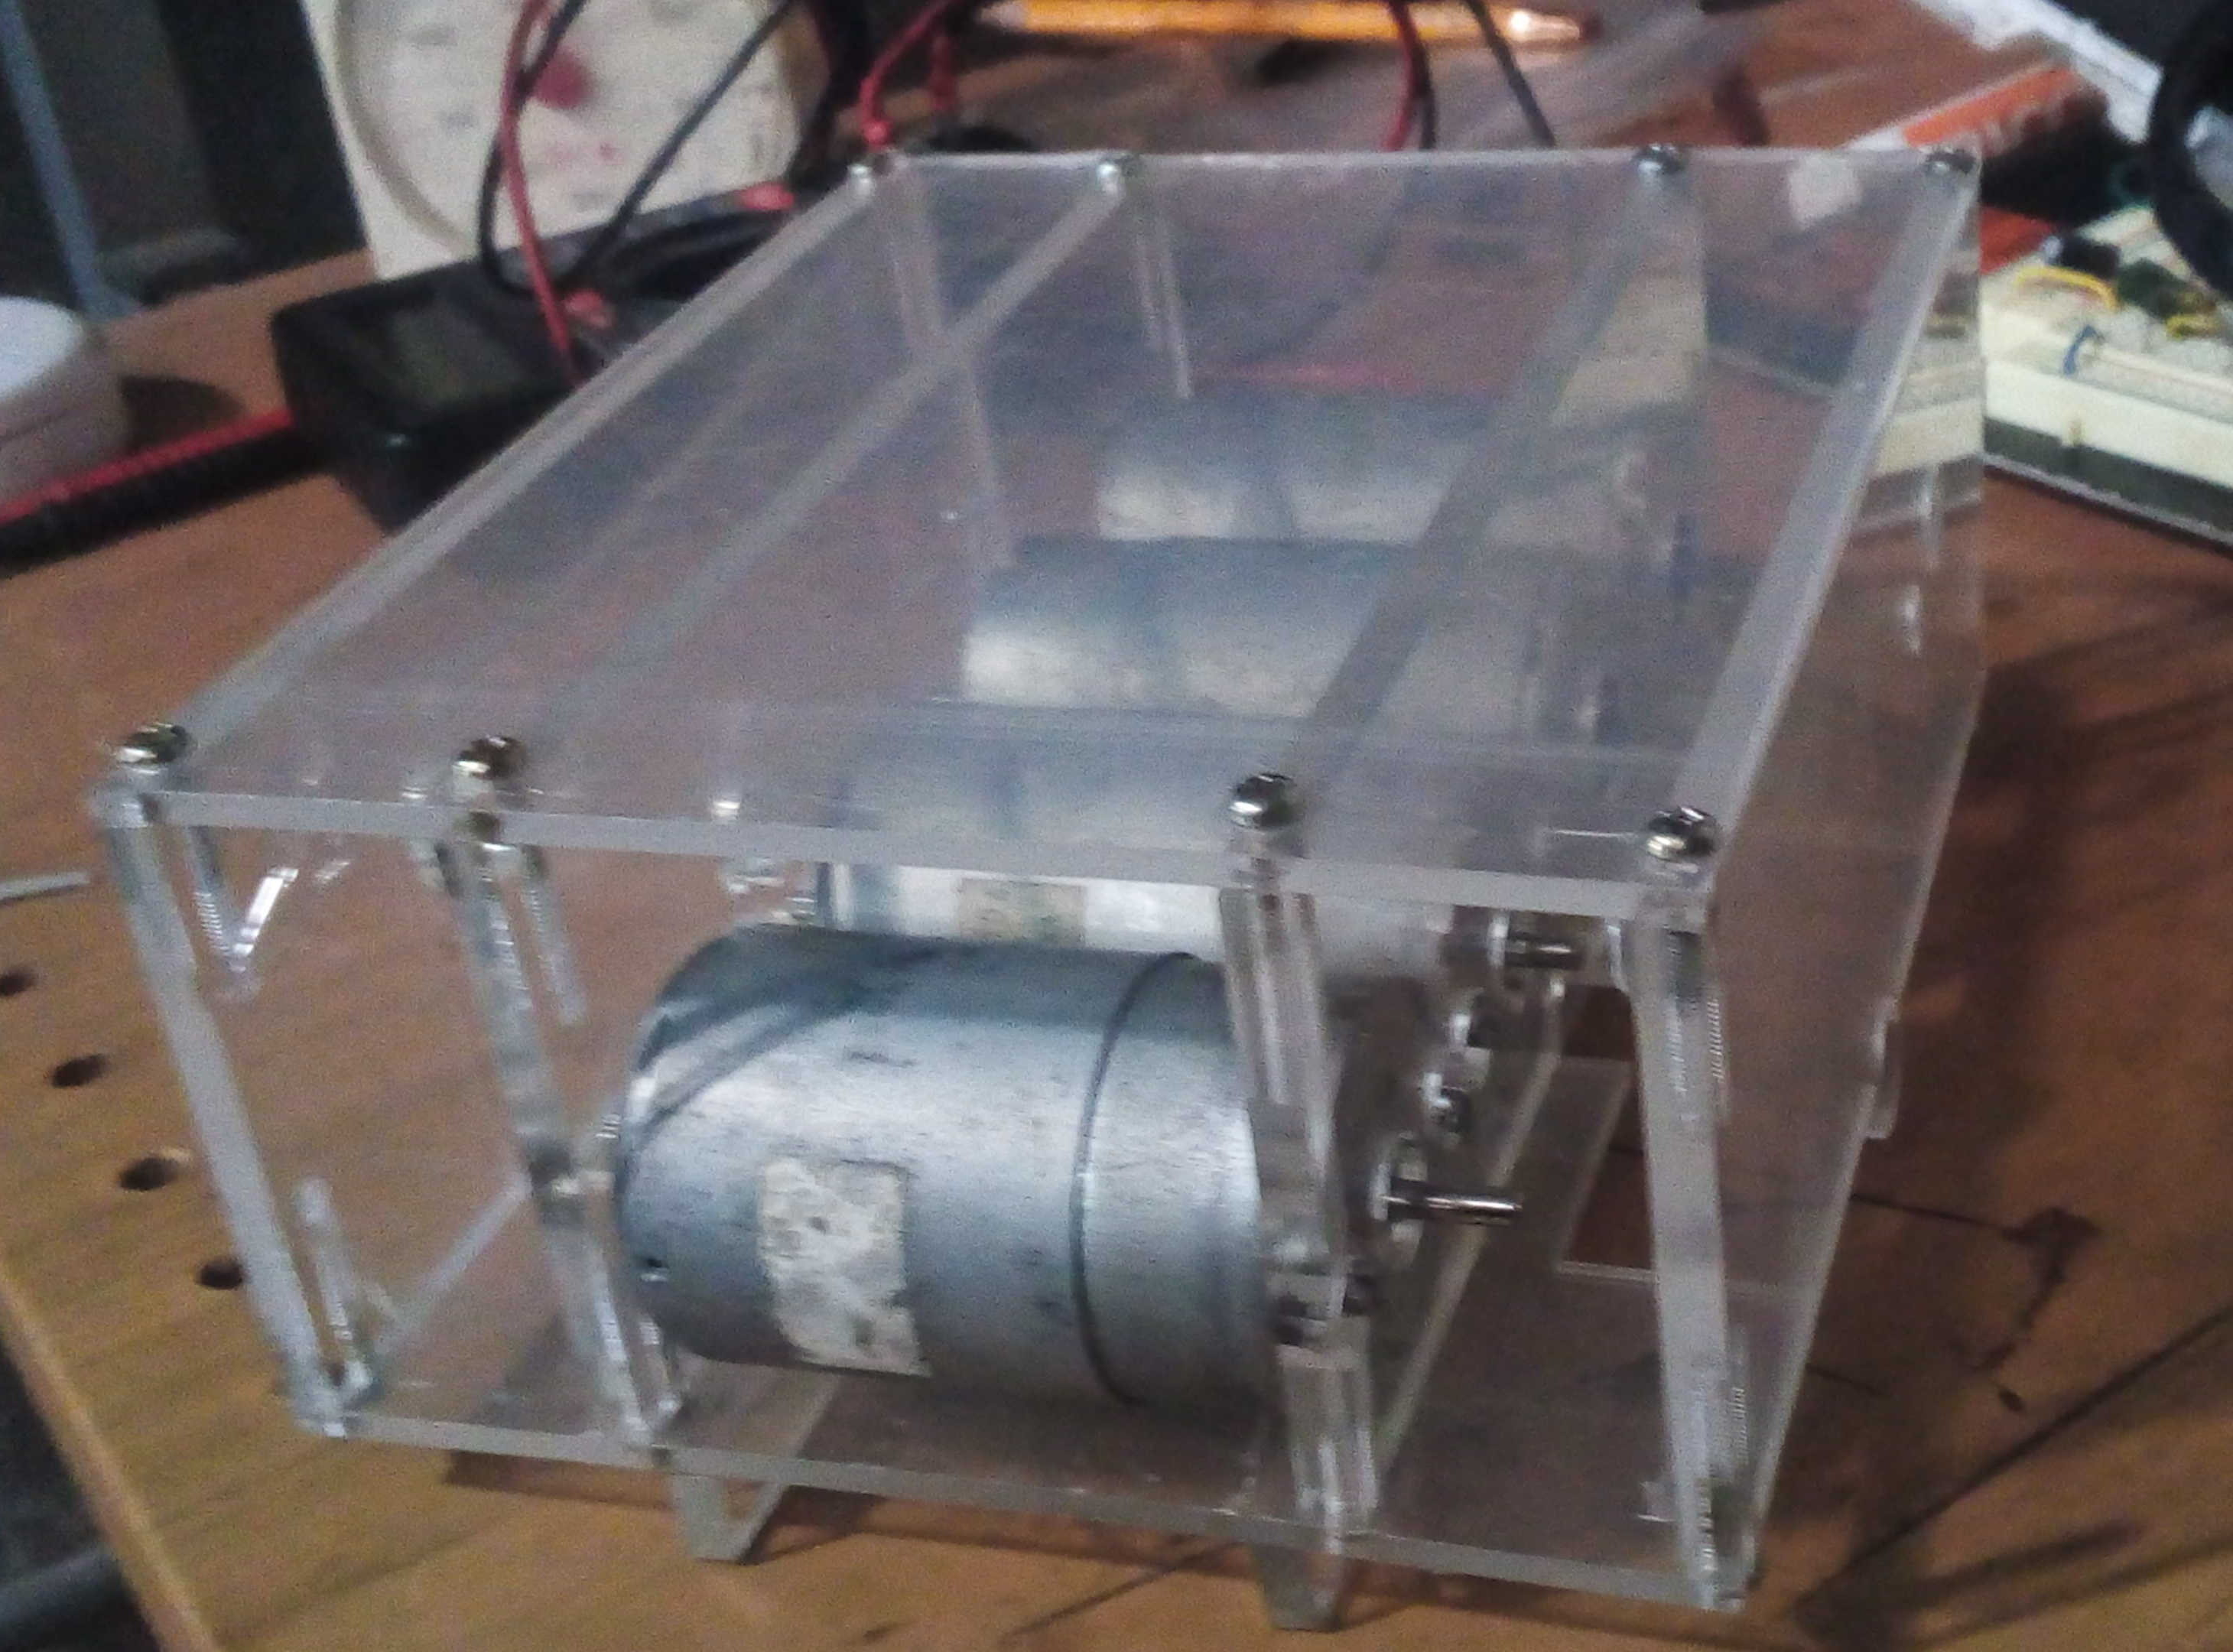
\includegraphics[width=0.4\linewidth]{imagenes/prototipo/CajaLista}

	\caption{Imagenes de armado del robot}
	\label{imagen:construccionFinalRobot}
\end{figure}



\subsection{Drivers}

Los drivers empleados en el diseño del robot fueron los STA6940M, los cuales soportan motores con escobillas con voltajes de operación de hasta 44V y 4 amperios de corriente promedio, y son compatibles con la tensión de alimentación lógica de 5V. La figura \ref{imagen:Driver} presenta el empaquetado 18-pin ZIP del driver empleado.

\begin{figure}[H]
	\centering		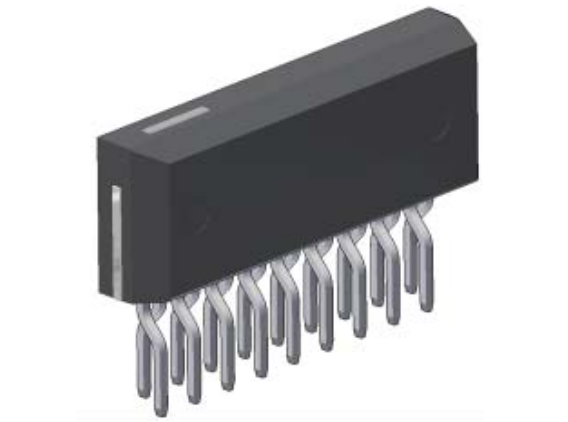
\includegraphics[width=0.3\linewidth]{imagenes/prototipo/Driver}
	\caption{Driver STA6940M. }
	\label{imagen:Driver}
\end{figure}

La configuración utilizada en el robot es similar a la recomendada por el fabricante en la figura \ref{imagen:DriverAplicacion}. El diagrama de pines se muestra en la tabla \ref{imagen:DriverTabla}.

\begin{figure}[H]
	\centering		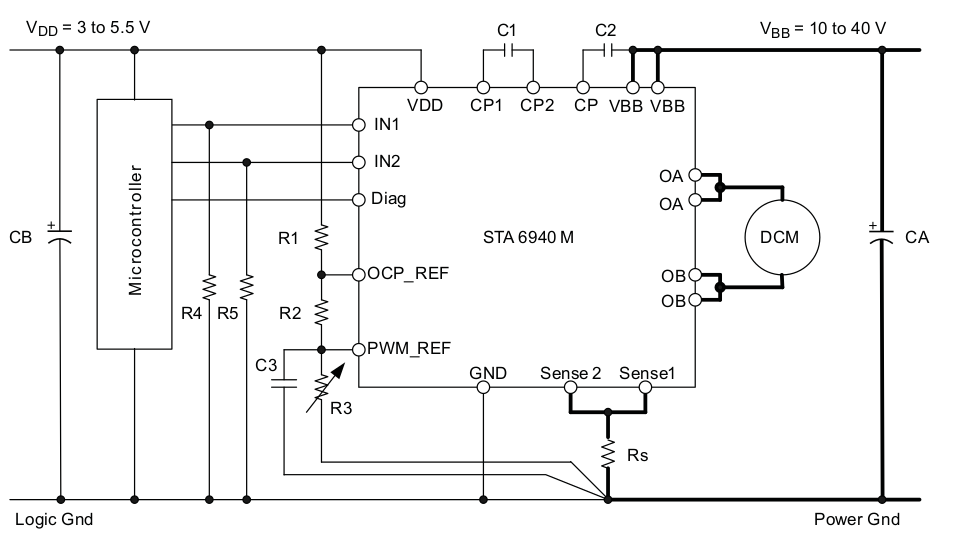
\includegraphics[width=0.7\linewidth]{imagenes/prototipo/InformacionDeAplicacion}
	\caption{Diagrama de aplicación del driver STA6940M proveído por el fabricante.}
	\label{imagen:DriverAplicacion}
\end{figure}


\begin{figure}[H]
	\centering		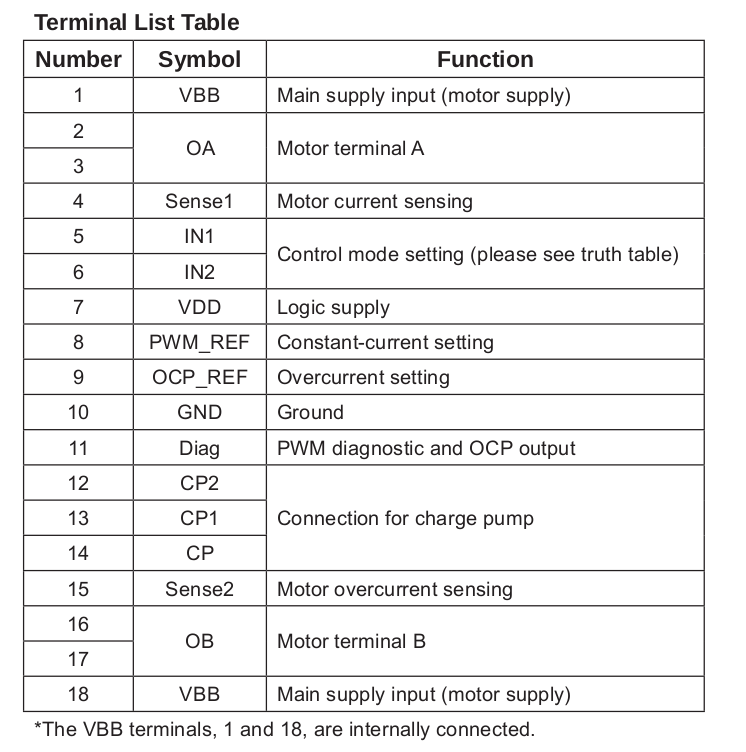
\includegraphics[width=0.7\linewidth]{imagenes/prototipo/TablaDePines}
	\caption{Lista de pines del driver STA6940M proveída por el fabricante. }
	\label{imagen:DriverTabla}
\end{figure}

Cabe destacar que la protección de sobrecorriente que presenta el driver ($OCP\_ REF$) es colacada manualmente con un arreglo de resisitencias ,al igual que la referencia del PWM ($PWM\_ REF$). En particular, el voltaje de $OCP\_ REF$ debe ser igual al voltaje de la resistencia de sensado cuando el motor presenta su punto de máximo torque, que en este caso es cuando se alcanza la corriente de Stall a 1.6 Amperios. En la configuración final se utilizan dos motores en paralelo para cada driver por lo que el ajuste se realizó para 3.2 Amperios.


\subsection{Encoders}

El sistema de encoders también fue diseñado desde cero. La figura \ref{imagen:RuedaEncoders} presenta el modelaje 3D de la rueda del encoder y la disposición final sobre el eje de la rueda del robot.

\begin{figure}[H]
	\centering		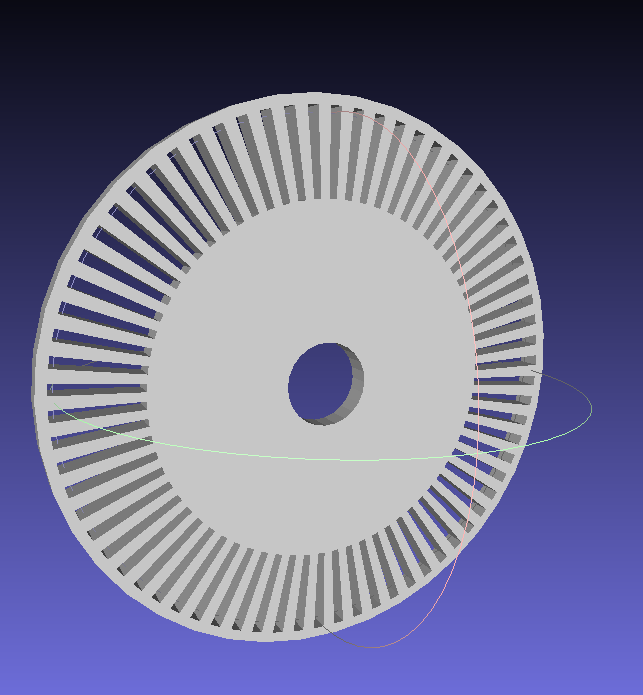
\includegraphics[width=0.3\linewidth]{imagenes/prototipo/Ruedaencoder}
	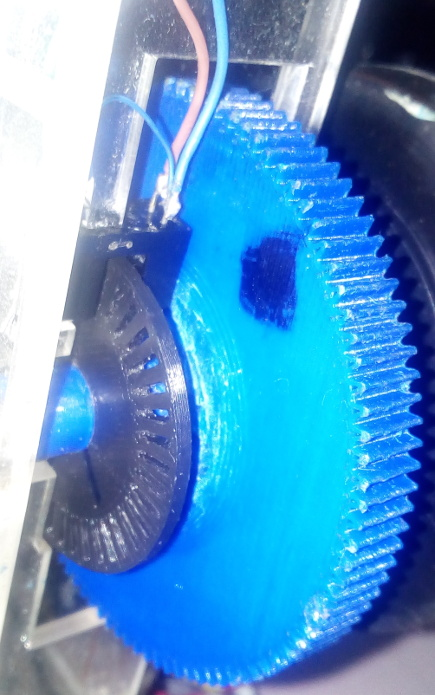
\includegraphics[width=0.3\linewidth]{imagenes/prototipo/EncoderReal}
	\caption{Diseño 3D de la rueda de los encoders del robot}
	\label{imagen:RuedaEncoders}
\end{figure}

El diseño final de la rueda del encoder tiene 40 ranuras. El proceso de calibración del encoder pasó por ajustar las resistencias de los fotoemisores y fotoreceptores del encoder y posteriormente realizar una restricción del mínimo tiempo de interrupción entre dos ranuras basada en la máxima velocidad de la rueda.

Cabe destacar que los encoders presentan un circuito de adecuación para generar la interrupciones en el microcontrolador de la placa de control a bajo nivel, el cual consiste en un comparador LM311.

Los resultados finales de calibración fueron bastantes satisfactorios, obteniéndose un error de lectura de 4 ranuras por cada 4000 ranuras, el cual representa un error de 0.1\%.
Cabe destacar que la correcta lectura de los encoders es de vital importancia para obtener datos confiables de odometría del robot.

\subsection{Placa de control a bajo nivel}
Los drivers del motor, los circuitos de acondicionamiento de los encoders y el microcontrolador encargado de realizar el control PWM del robot fueron integrados en una PCB, la cual se diseño utilizando Kicad 5.0.2 para Ubuntu. La figura \ref{imagen:PlacaMotores} presenta el esquemático de la placa. El microcontrolador utilizado fue el Arduino Nano 328p.


\begin{figure}[H]
	\centering		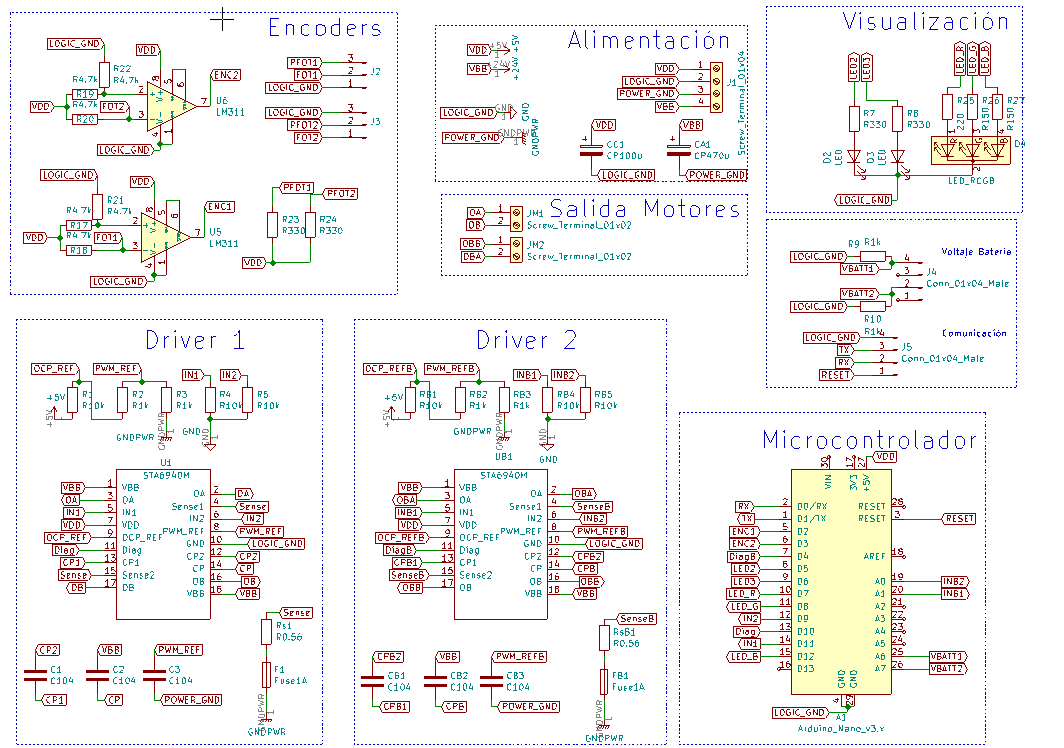
\includegraphics[width=1.0\linewidth]{imagenes/prototipo/Placa/PlacaMotores}
	\caption{Esquemático de la placa de los motores.}
	\label{imagen:PlacaMotores}
\end{figure}

Las figura \ref{imagen:PlacaMotoresFrontal} presenta la vista frontal de las capas de la placa, su vista 3D y el modelo final.


%\begin{figure}[H]
%	\centering		
%	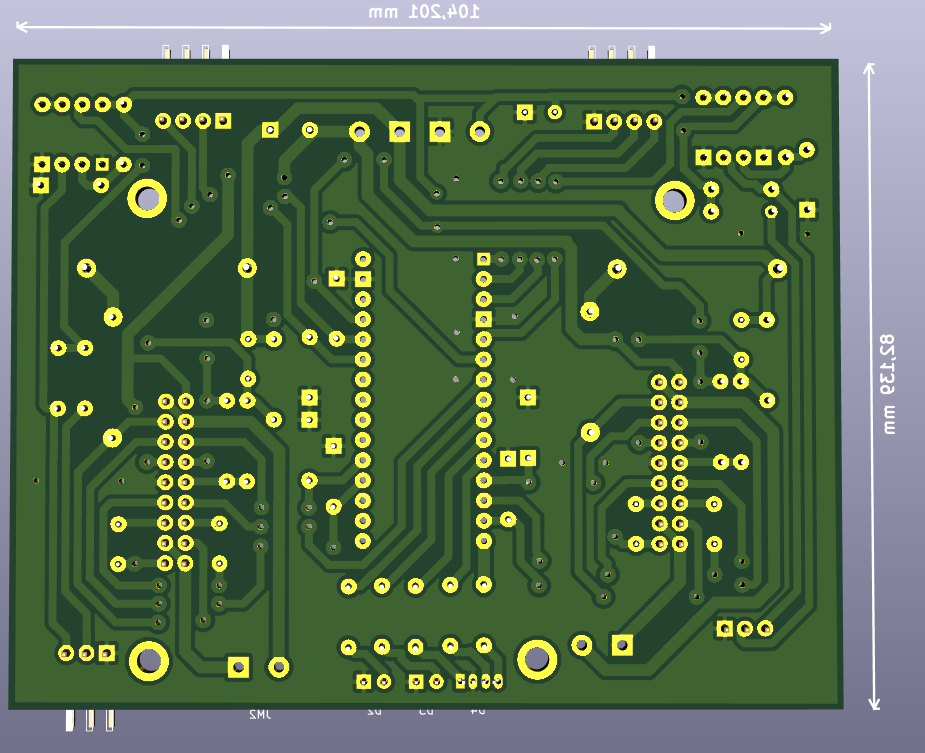
\includegraphics[width=0.7\linewidth]{imagenes/prototipo/Placa/3dViewerBottom}
%	\caption{Vista trasera de las capas de la placa de los motores}
%	\label{imagen:PlacaMotoresBottom}
%\end{figure}


\begin{figure}[H]
	\centering	
	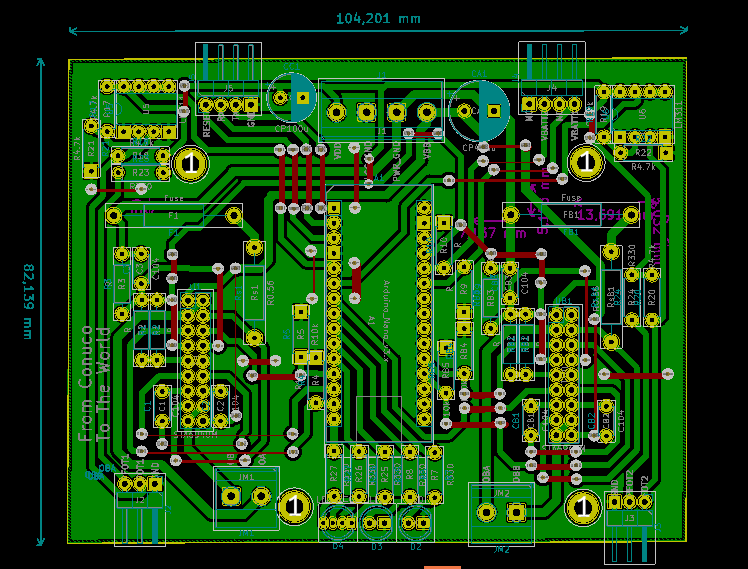
\includegraphics[width=0.7\linewidth]{imagenes/prototipo/Placa/PCB_FrontAllLayers}	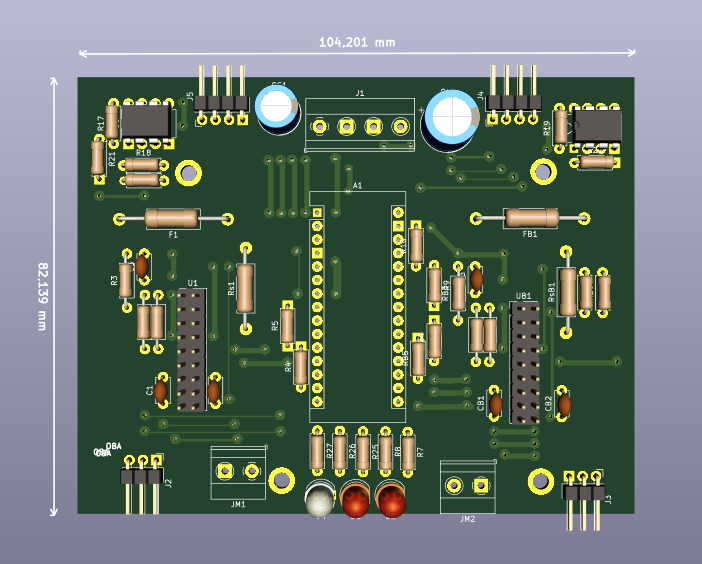
\includegraphics[width=0.7\linewidth]{imagenes/prototipo/Placa/3dViewerFront}
	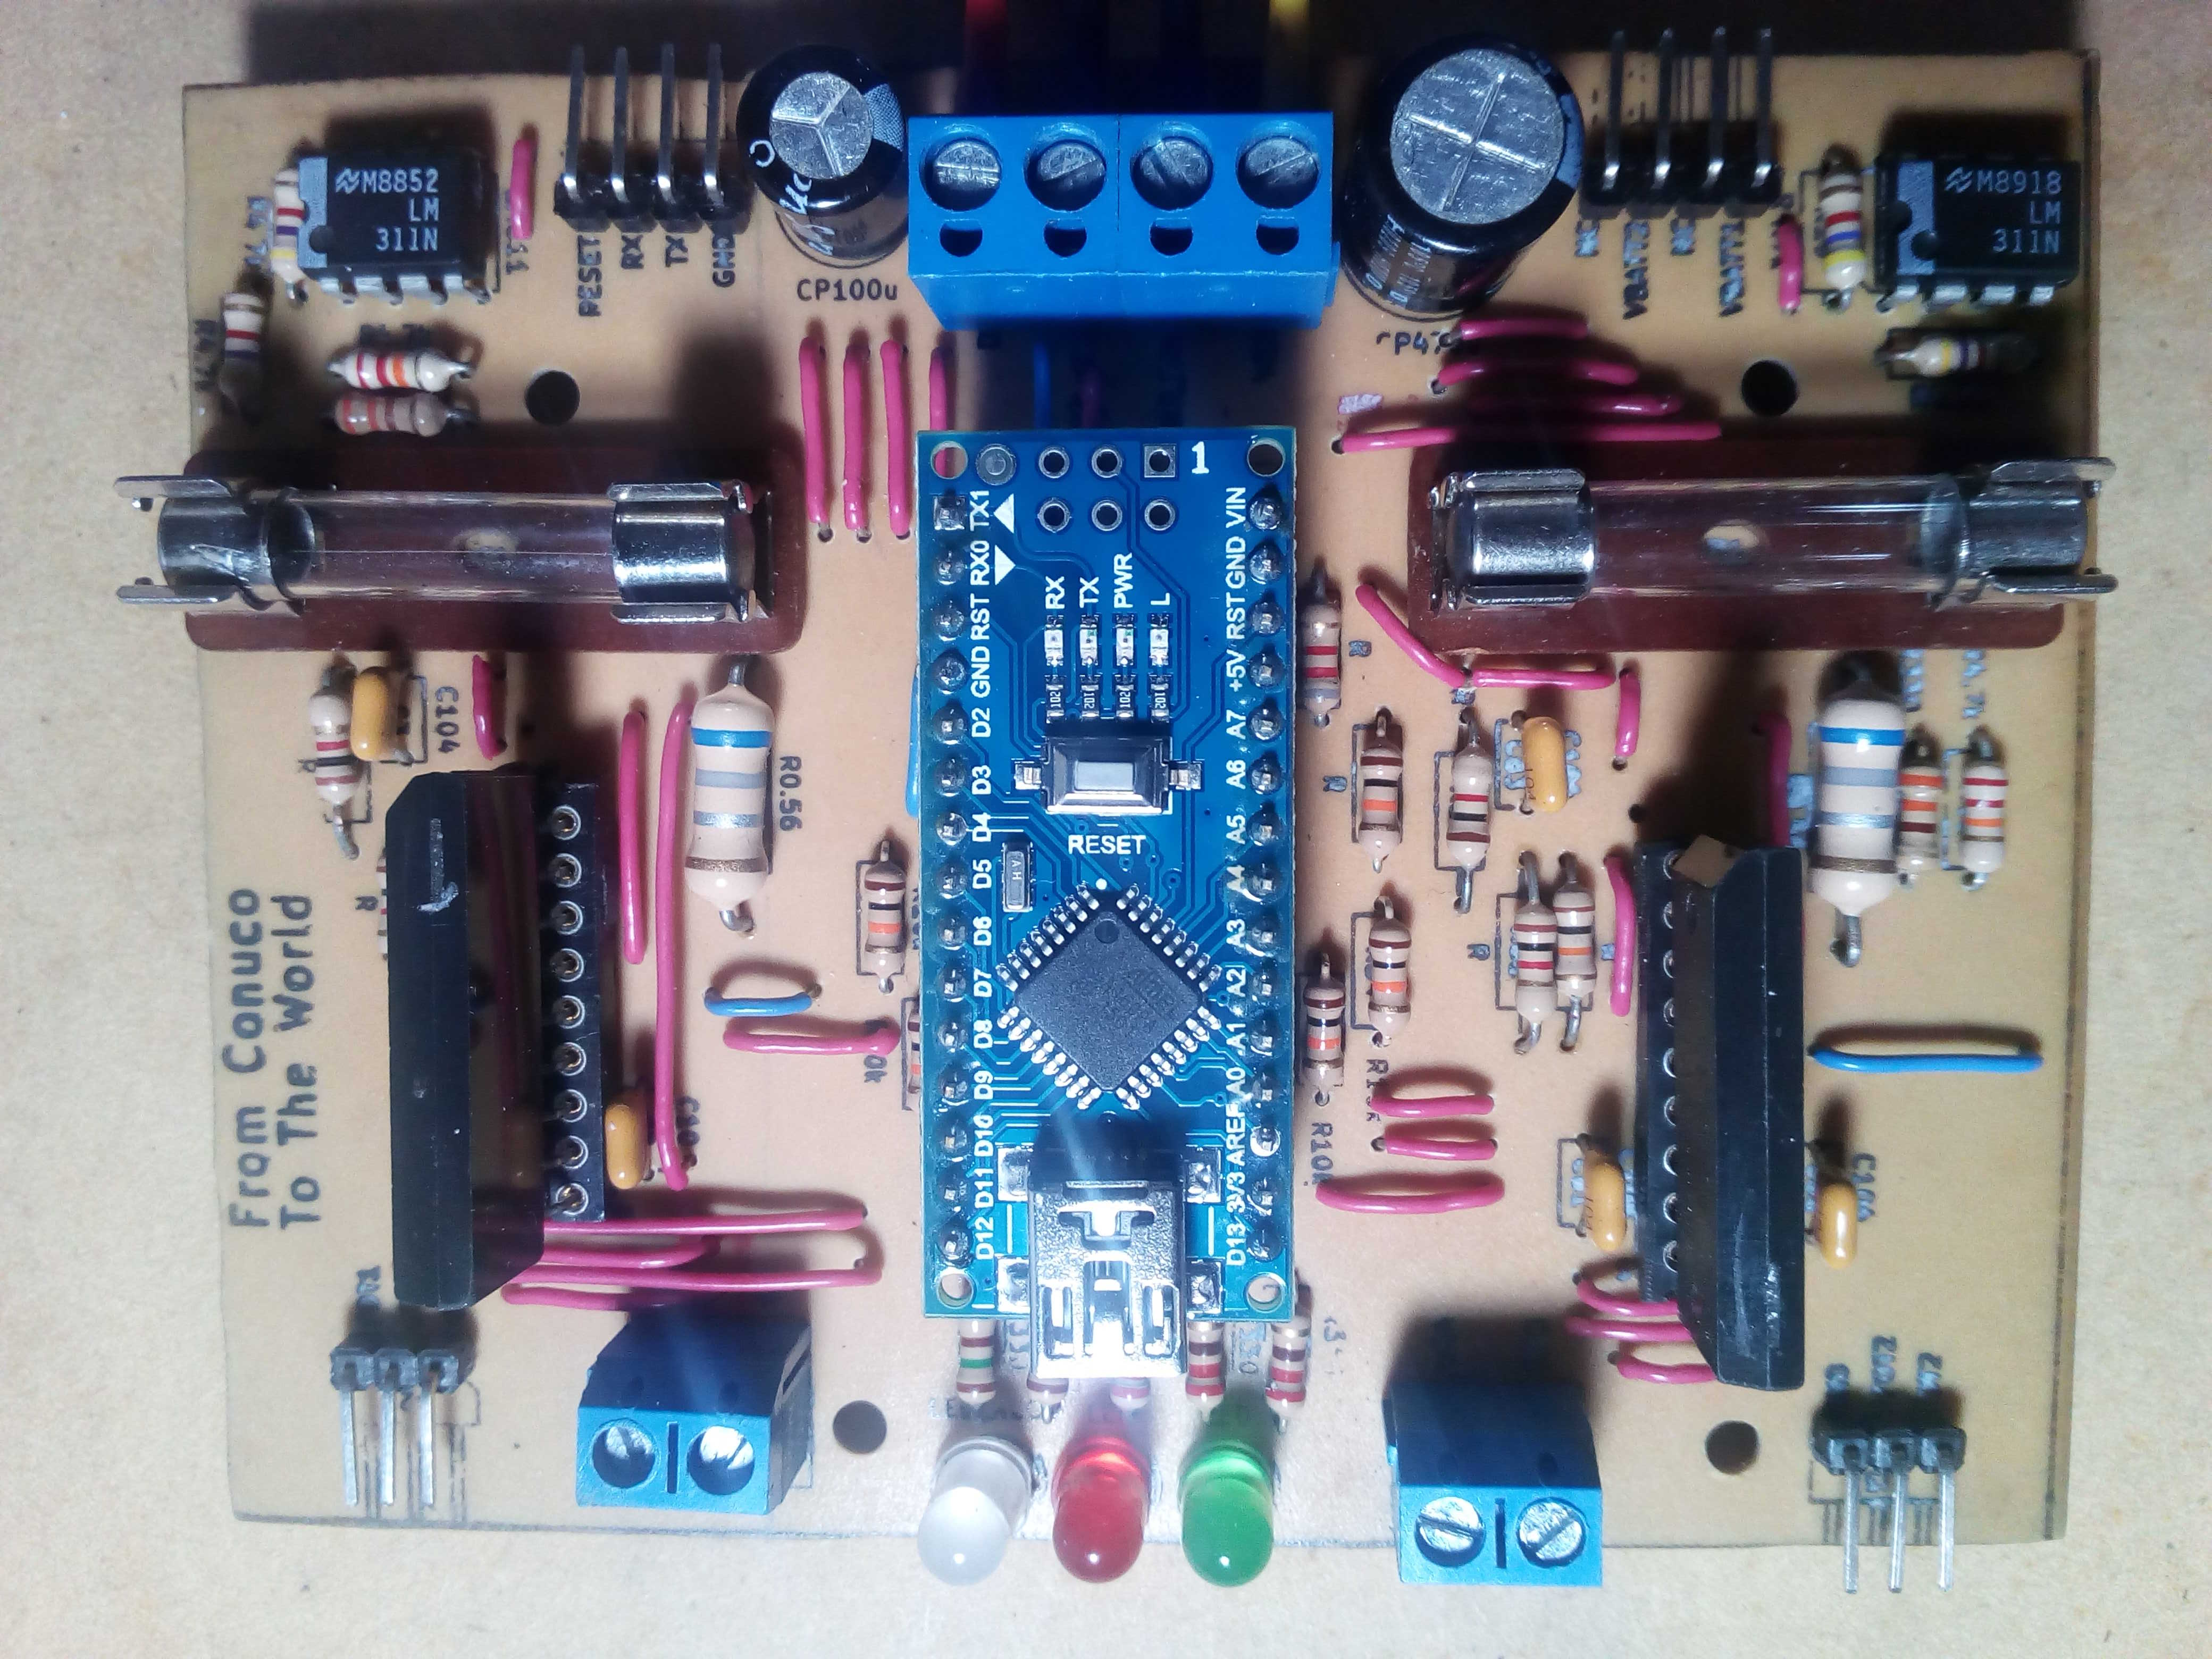
\includegraphics[width=0.7\linewidth]{imagenes/prototipo/Placa/PCB_FinalFront}
	\caption{Vista frontal de la placa de los motores.}
	\label{imagen:PlacaMotoresFrontal}
\end{figure}

\subsection{Sistema de alimentación y autonomía}

El robot es alimentado por dos paquetes de baterías de 12V, los cuales fueron construidos con baterías de litio Sony G5 18650 de 2200mAh. Cada paquete dispone de 6 baterias de litio, para un total de 12 baterías.  Estas baterías se disponen en serie para lograr el voltaje de 24V de funcionamiento de los motores del robot, con una capacidad de 4400mAh. Se aprovecha la toma de 12V para alimentar la placa de control de los motores y la raspberry utilizando dos conversores del tipo Buck independientes. Los conversores empleados son del tipo MP2307, y su voltaje de salida es fijado a  5V.
La figura \ref{imagen:BuckCurva} presenta la curva de eficiencia del conversor utilizado.


\begin{figure}[H]
	\centering	
	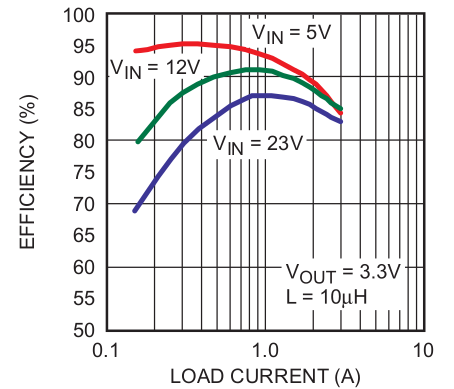
\includegraphics[width=0.5\linewidth]{imagenes/prototipo/Buck}
	\caption{Curva de eficiencia vs corriente de carga del conversor Buck utilizado}
	\label{imagen:BuckCurva}
\end{figure}


En la figura \ref{imagen:Bateria} se presenta el proceso de carga de uno de los paquetes de batería de 12V. En este caso se utilizan 3 circuitos de cargadores de batería de litio de 3.7V HW-107 que emplean el controlador de carga TC4056. Estos circuitos se encuentran eléctricamente aislados ya que utilizan cargadores independientes de la red eléctrica nacional a 5V@1A. El tiempo aproximado de carga de cada paquete de batería es de 6 horas.

\begin{figure}[H]
	\centering	
	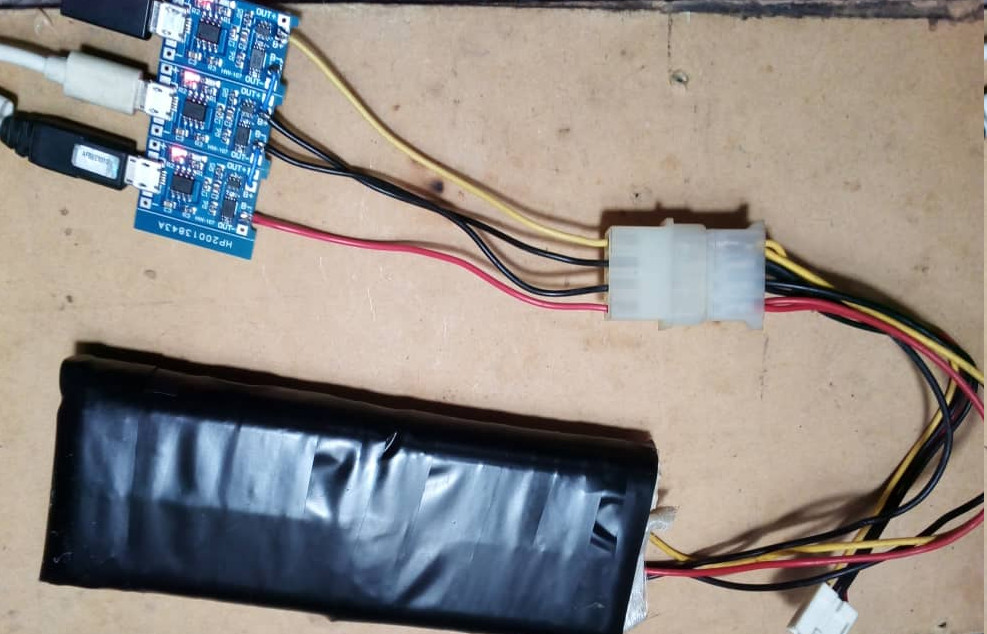
\includegraphics[width=0.7\linewidth]{imagenes/prototipo/Bateria}
	\caption{Carga del paquete de baterías de 12V del robot.}
	\label{imagen:Bateria}
\end{figure}

También se presenta el cálculo de autonomía del robot en función de la eficiencia de los conversores tipo Buck y del consumo de los componentes del robot.

La tabla \ref{Buck1} presenta el consumo de carga promedio del conversor Buck 1. En este caso la corriente de carga aproximada es de 115.2 mA, y debido a que el voltaje de salida es de 5V, la potencia de consumo es 0.58 W. En esta caso se aproxima la eficiencia del conversor a 90\% para el cálculo de las perdidas de conversión. La tabla \ref{Buck1Perdidas} presenta la corriente de alimentación suminastrada por el arreglo de baterías de 12V en el proceso de conversión, la cual es la potencia total consumida por el conversor entre 12V.

\begin{table}[htbp]
	\caption{Consumo de carga del conversor Buck 1}
	\begin{tabular}{|l|c|c|c|c|}
		\hline
		\multicolumn{1}{|c|}{\textbf{Componente}} & \textbf{Cantidad} & \textbf{ Vin (V)} & \textbf{ Ipr (mA)} & \textbf{Itotal (mA)} \\ \hline
		Arduino Nano 328p & 1 & 5 & 15 & 15 \\ \hline
		Leds PCB & 3 & 5 & 10 & 30 \\ \hline
		Fotoreceptor-Fotoemisor Encoder & 2 & 5 & 10 & 20 \\ \hline
		Comparador LM311 & 2 & 5 & 5.1 & 10.2 \\ \hline
		Driver STA6940M & 2 & 5 & 20 & 40 \\ \hline
		& \multicolumn{1}{l|}{} & \multicolumn{1}{l|}{} & \textbf{Iload (mA)} & 115.2 \\ \hline
	\end{tabular}
	\label{Buck1}
\end{table}



\begin{table}[htbp]
	\caption{Consumo conversor Buck 1}
	\begin{tabular}{|l|c|}
		\hline
		Consumo Buck 1 (W) & 0.58 \\ \hline
		Perdidas por Conversión (W) & 0.06 \\ \hline
		Consumo Total (W) & 0.64 \\ \hline
		Corriente de Alimentación Equivalente (mA) & \multicolumn{1}{r|}{53.3333333333} \\ \hline
	\end{tabular}
	\label{Buck1Perdidas}
\end{table}


En el caso del consumo del conversor Buck 2, se calcula  en función del consumo promedio de la Raspberry Pi 3 utilizando sus cuatro núcleos al 100\%, el consumo de la cámara y el de la IMU. La tabla \ref{} presenta estos resultados.

\begin{table}[htbp]
	\caption{Consumo conversor Buck 2}
	\begin{tabular}{|l|c|c|c|c|}
		\hline
		\multicolumn{1}{|c|}{\textbf{Componente}} & \textbf{Cantidad} & \textbf{ Vin (V)} & \textbf{ Ipr (mA)} & \textbf{Itotal (mA)} \\ \hline
		IMU MPU6050 & 1 & 3.3 & 3.8 & 3.8 \\ \hline
		Raspberry Pi 3  & 1 & 5 & 730 & 730 \\ \hline
		Pi Camera  v1.2 & 1 & 1.3 & 250 & 250 \\ \hline
		& \multicolumn{1}{l|}{} & \multicolumn{1}{l|}{} & \textbf{Iload (mA)} & 983.8 \\ \hline
	\end{tabular}
	\label{Buck2}
\end{table}

\begin{table}[htbp]
	\caption{Consumo conversor Buck 2}
	\begin{tabular}{|l|c|}
		\hline
		Consumo Buck 2 (W) & 1.3 \\ \hline
		Perdidas por Conversión (W) & 0.54 \\ \hline
		Consumo Total (W) & 5.4 \\ \hline
		Corriente de Alimentación Equivalente (mA) & 450 \\ \hline
	\end{tabular}
	\label{Buck2Perdidas}
\end{table}

Por tanto el consumo de corriente total de los Bucks es de  503mA, a lo cual se le debe sumar los 250mA estimados que consume en promedio cada motor del robot. Por tanto el consumo total del robot es de 1.5A, por paquete de baterías. Como cada paquete presente una capacidad de 4400 mAh, la autonomía estimada es de aproximadametne 2 horas. Sin embargo, la autonomía real del robot es de aproximadamente 1 hora debido a que las baterías empleadas son recicladas.



\section{Componentes de hardware}
En la figura \ref{imagen:HardwareRobot} se presenta el hardware base utilizado para la creación del dataset visual inercial.

La cámara y la imu forman parte de los sensores empleados para la recopilación de información, mientra que el microcontrolador Arduino forma parte de la placa de control del robot y posee información de odometría del mismo. La Raspberry es utilizada para guardar la información suminstrada por los sensores y como medio de interconexión del control de mando.

\begin{figure}[H]
	\centering
	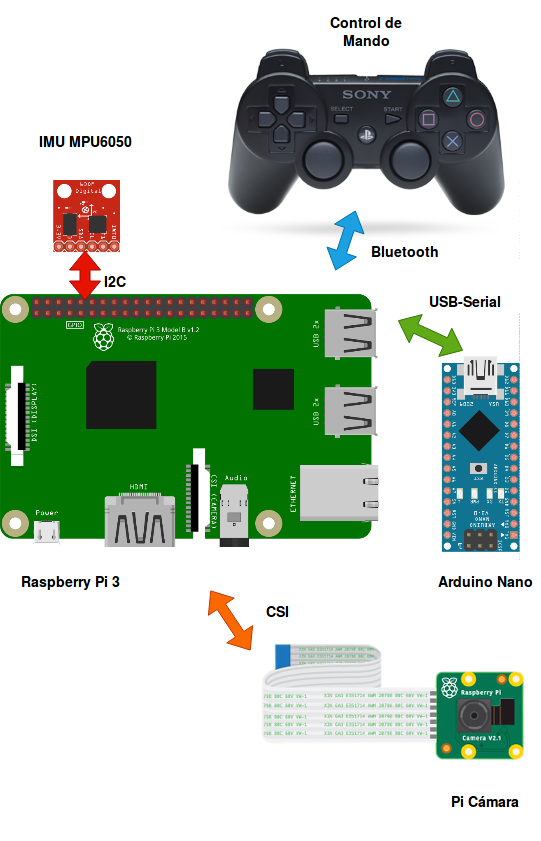
\includegraphics[width=0.7\textwidth]{HardwareRobot}
	\caption[Componentes de Hardware del robot]{Componentes de Hardware del robot.}
	\label{imagen:HardwareRobot}
\end{figure}

\subsection{Joystick}

En la figura \ref{imagen:Joystick} se presenta el mapa de los botones del robot. En esta implementación el control de mando es utilizado para el movimiento del robot y para el inicio y finalización de las secuencias del dataset local visual-inercial.

\begin{figure}[H]
	\centering	
	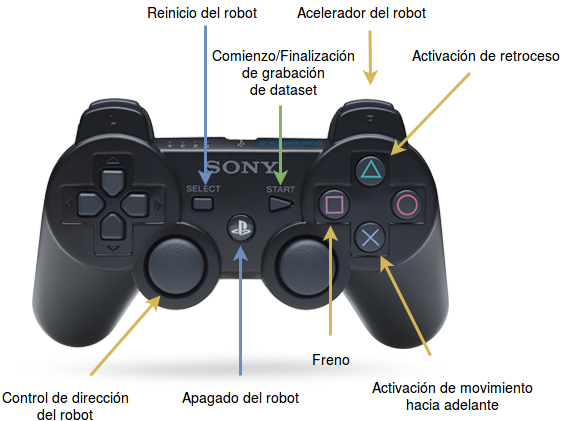
\includegraphics[width=0.7\linewidth]{imagenes/prototipo/Joystick}
	\caption{Mapeo de botones del control de mando.}
	\label{imagen:Joystick}
\end{figure}

\subsection{Cámara}

La cámara utilizada para el prototipo fue la Pi Camera v1.2, la cual se conecta a la Raspberry P utiilzando la interfaz CSI, la cual provee un ancho de banda de 2Gbps .Esta cámara permite capturar imágenes con resoluciones de hasta 2592x1944 a 15Hz, y capturar movimientos rápidos a 90Hz con una resolución de 640x480.

La cámara es controlada por la GPU de la Raspberry. Las funciones de postprocesamiento como el balance de blancos, ganancia digital, procesamiento de color, redimensionamiento de la imagen, entre otras, son ejecutadas en la GPU en su propio sistema de tiempo real ThreadX. La configuración de la frecuencia de muestreo de la cámara y funciones de postprocesamiento se coloca mediante la configuración de registros.La GPU posee una memoria asignada de 128MB en la memoria ram de la Raspberry, la cual es utilizada como buffer de imágenes. 

El CPU uiliza el VCHI (del inglés: VideoCore Host Interface) para comunicarse con la GPU mediante el envio de mensajes. Para utilizar la GPU y la cámara de la Raspberry lenguajes como Python y C++ utilizan la librería MMAL (del inglés: Multimedia Abstraction Layer) la cual es diseñada por Broadcom para utilizar la GPU Videocore IV de la Raspberry Pi de una forma más sencilla para programadores. De esta forma, los mensajes de configuración y de lectura de datos son gestionados por la MMAL que utiliza el VCHI para enviarlos a la GPU.

La figura \ref{imagen:ArquitecturaCamara} presenta la flujo de la arquitectura para capturar imagen o video en Python. Cabe destacar que el puerto MMAL genera una excepción (callback en la figura) cuando una nueva imagen se encuentra disponible en RAM. Esto fue de vital importancia para la generación del dataset, ya que esta excepción se utiliza como disparo para realizar los demás procesos involucrados como por ejemplo la lectura de la imu, manteniendo la sincronización.


\begin{figure}[H]
	\centering		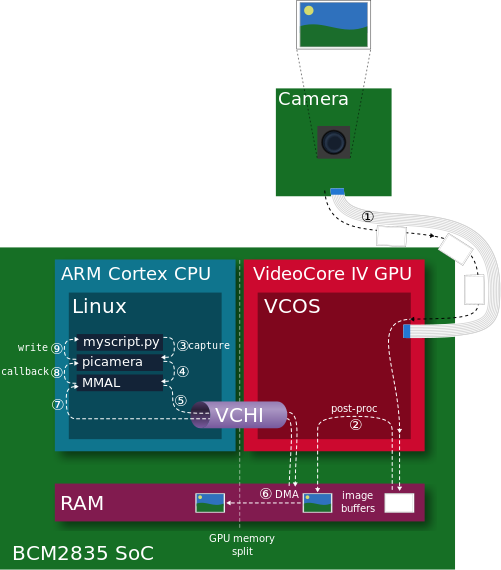
\includegraphics[width=0.7\linewidth]{imagenes/prototipo/camera_architecture}
	\caption{Arquitectura de la cámara en la Raspberry. Obtenido de\protect\footnotemark.}
	\label{imagen:ArquitecturaCamara}

\end{figure}
\footnotetext{\url{https://picamera.readthedocs.io/en/release-1.13/fov.html}}

El código empleado para la gestión de la camera en el dataset se realizó en  utilizando un API en C++ desarrollado por el grupo de investigacion AVA\protect\footnotemark. En este caso, la máxima resolución disponible es de 1280x960.

\footnotetext{\url{https://github.com/cedricve/raspicam}}


\subsection{IMU}

La imu utilizada fue la MPU6050, la cual incorpora un giroscopio y acelerometro de 3 ejes. Posee un buffer FIFO de 1024 Bytes y es compatible con el protocolo  I2C. Utiliza conversores analogico-digitales de 16-bits para digitalizar las mediciones del giroscopio y del acelerómetro, empleando un conversor por eje, lo que da un tamaño base de paquete de 12 Bytes para las lecturas de velocidad angular y aceleración. También dispone de un sensor de temperatura que en este caso no es utilizado. 
Cuando el sensor de temperatura no es utilizado, el buffer de la imu es capaz de guardar cerca de 85 medidas del giroscopio y acelerómetro que pueden ser posteriormente leidas en rafagas para su procesamiento. Esta característica es realmente importante a medida que la frecuencia de muestreo de la IMU aumenta, ya que permite el almacenamiento temporal de las medidas mientras el dispositivo maestro se encuentra realizando otras operaciones, lo cual es consistente en el caso de la Raspberry ya que al ejecutar un sistema operativo no es capaz de mantener el sincronismo de operaciones a frecuencias muy elevadas ( mayores a 100Hz).

La escala de medición es programable. El acelerómetro tiene rangos de $\pm$2g, $\pm$4g, $\pm$8g y $\pm$16g, mientras que el giroscópio tiene un escala de $\pm$250, $\pm$500, $\pm$1000, y $\pm$2000 °/s (DPS).

La MPU6050 posee un oscilador interno que provee la fuente de la frecuencia de muestreo y no permite una fuente de reloj externa para sincronizar estas medidas con la cámara. Este es un punto a destacar con respecto al EuRoc MAV Dataset, ya que en este último si se utiliza una fuente global de reloj que permite el sincronismo de las lecturas de las imágenes de la cámara y de la unidad de medición inercial. Sin embargo, al elevar la frecuencia de muestreo de la IMU a 10 veces más que la de la cámara, se puede utilizar la aproximación de que la primera y ultima de las medidas se encuentran lo suficientemente cercanas en tiempo al momento de captura de la imágenes. De no cumplirse esto, existirian mayores errores de residuales de rotación y de aceleración  entre imágenes.
 

\subsection{Disposición de sensores visuales inerciales}

En la figura \ref{imagen:Raspbery} se presenta la   y la imu MPU6050 conectadas a la Raspberry Pi 3.  La matriz de transformación de la cámara a la imu fue calculada de forma aproximada.



\begin{figure}[H]
	\centering		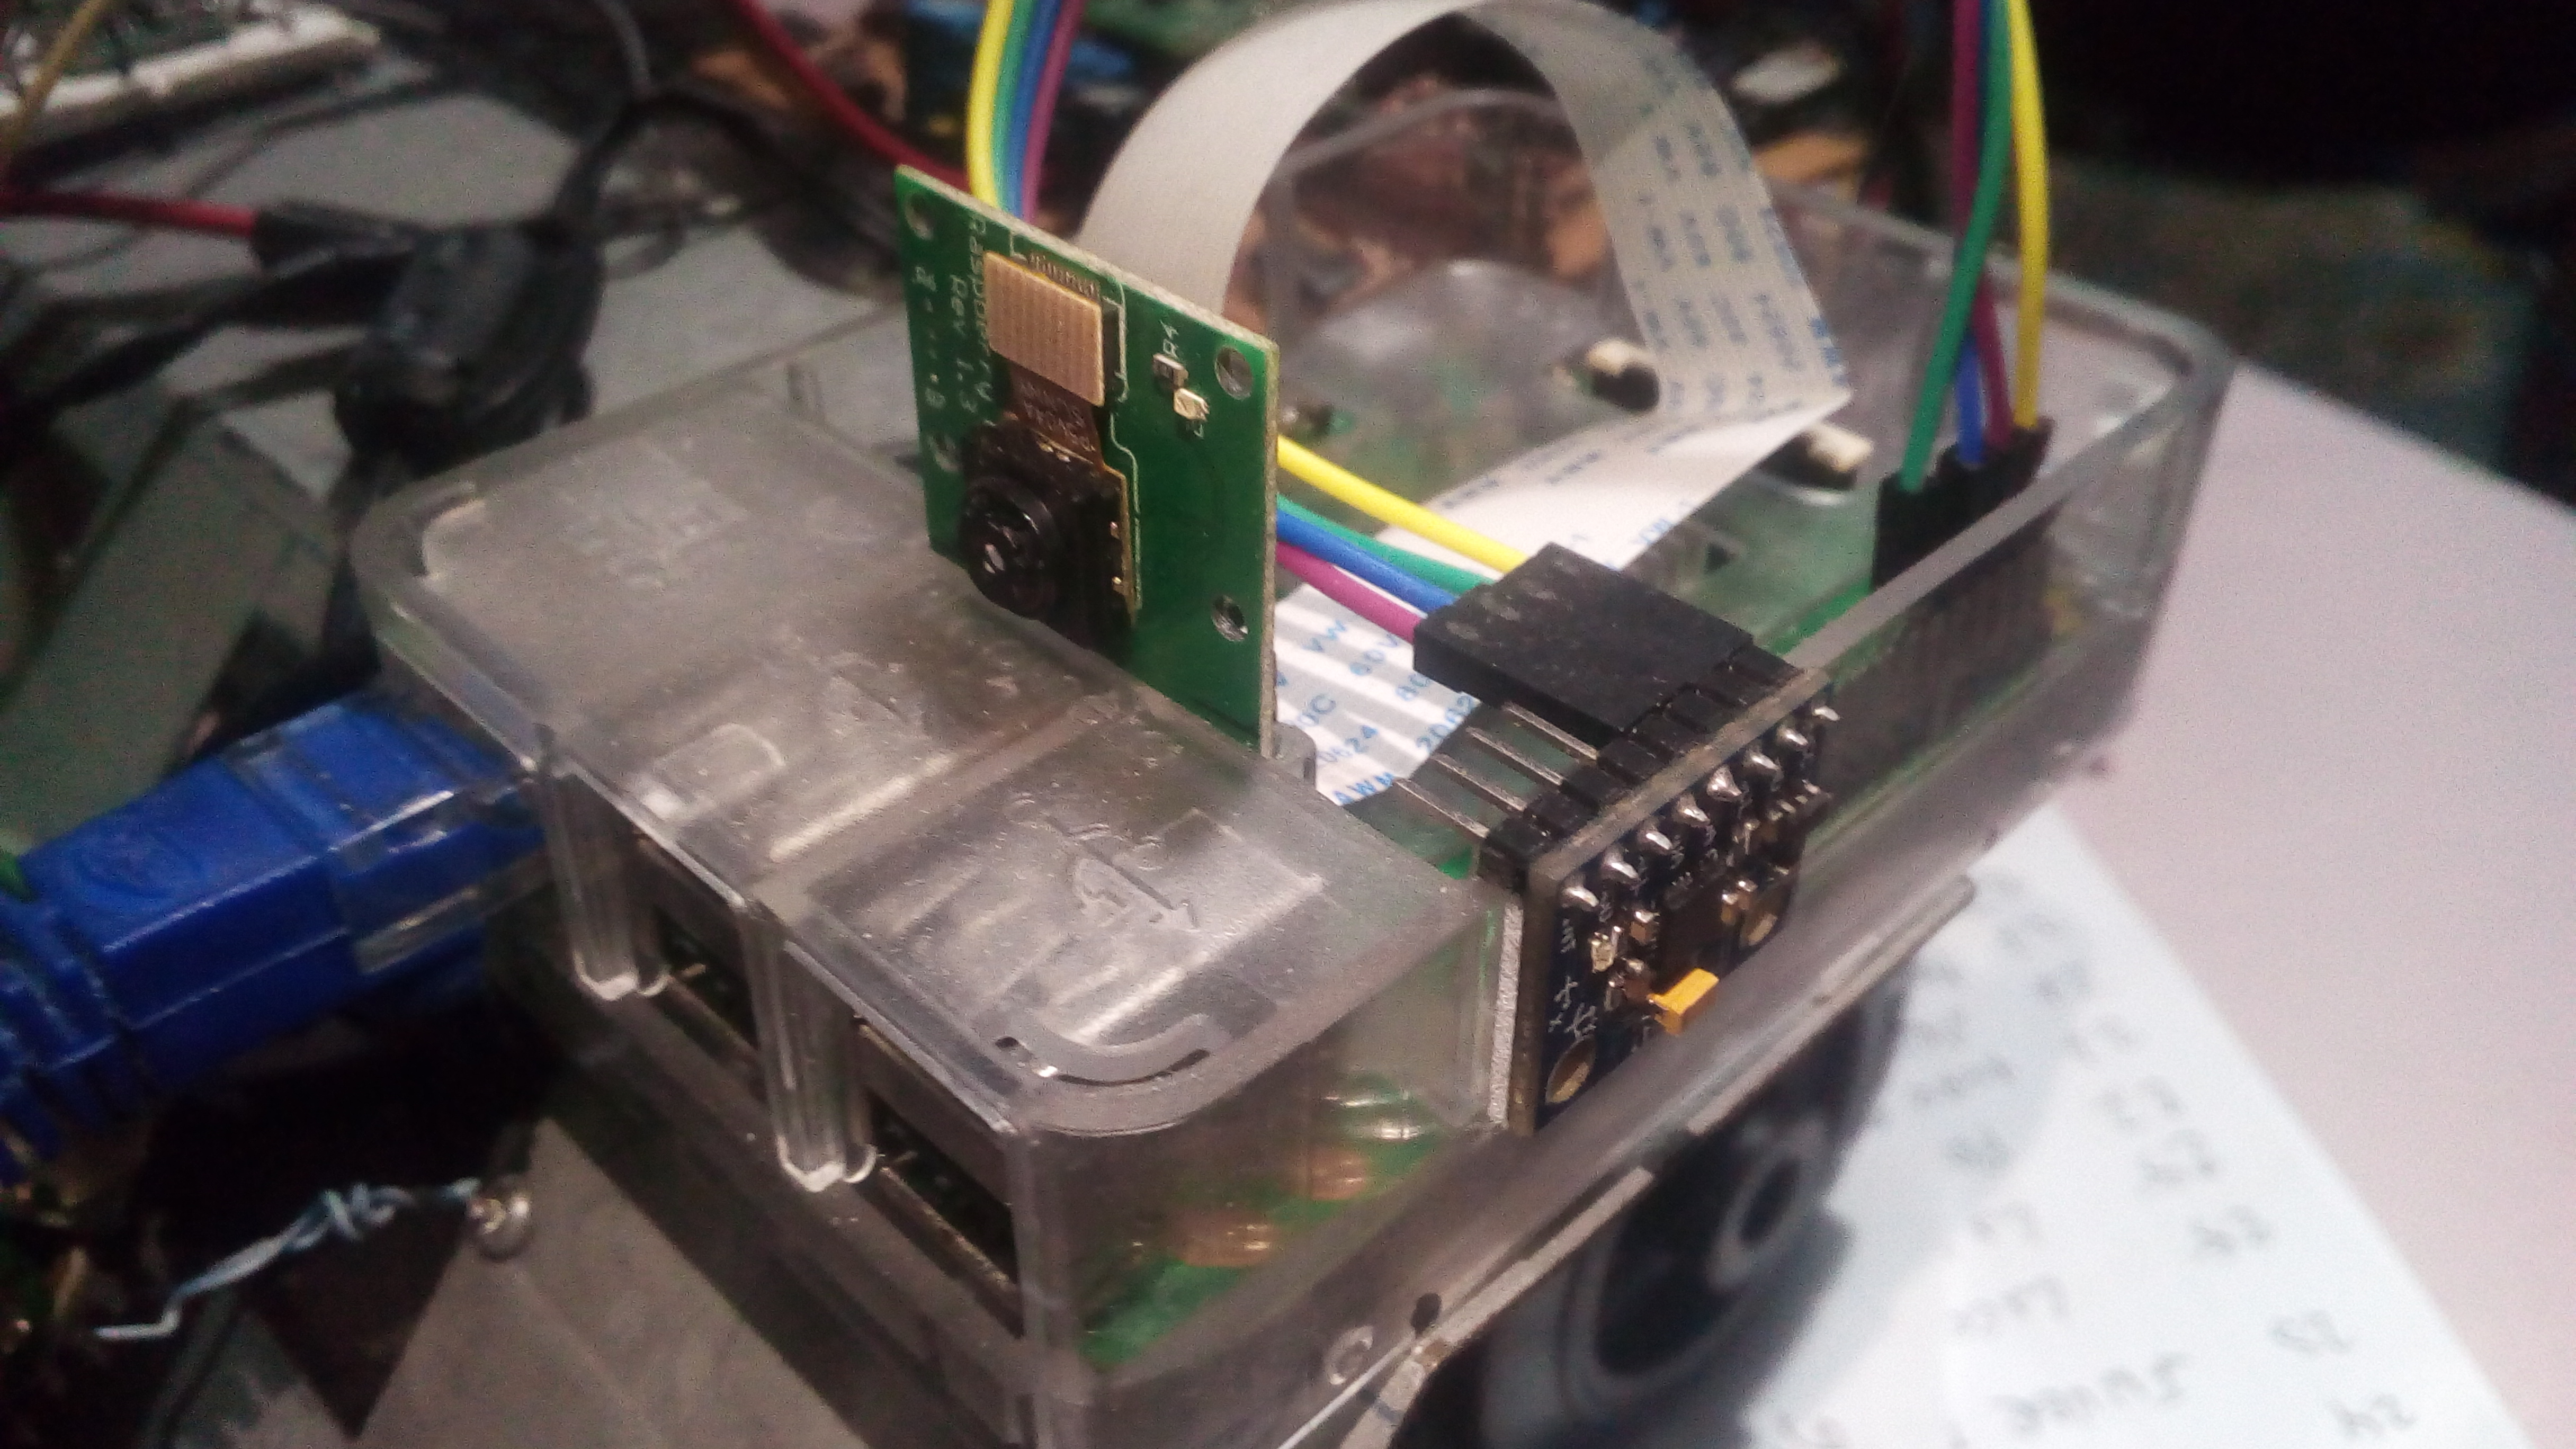
\includegraphics[width=0.7\linewidth]{imagenes/prototipo/Raspberry}
	\caption{Disposición de sensores en la Raspberry Pi 3}
	\label{imagen:Raspbery}
\end{figure}


\subsection{Raspberry Pi 3 y dataset local}

El dataset local realizado fue implementado utilizando C++ como lenguaje de programación, y empleando una Raspberry Pi 3 para la adquisición de los datos de la imu y de la cámara, y utilizando 4 hilos de ejecución.

El diagrama de la figura \ref{imagen:diagramaMultithread} presenta el esquema basico de la distribución de tareas entre hilos.

\begin{figure}[H]
	\centering
	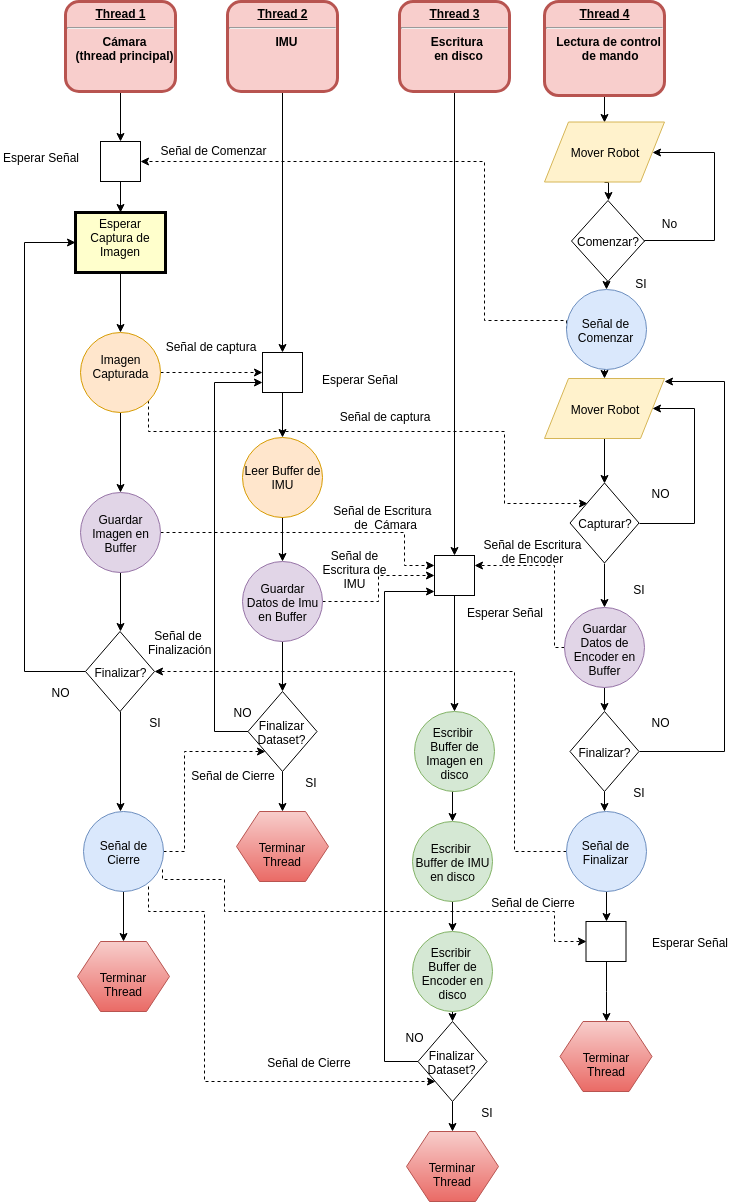
\includegraphics[width=1.0\linewidth]{imagenes/Implementacion/DiagramaMultithread}
	\caption{Diagrama de la programación multihilo del dataset visual inercial}
	\label{imagen:diagramaMultithread}
\end{figure}

\subsection{Presupuesto de datasets visuales inerciales}



\begin{table}[htbp]
	\caption{Presupuesto del robot prototipo}
	\begin{tabular}{|l|c|c|c|}
		\hline
		\multicolumn{1}{|c|}{\textbf{Componente}} & \textbf{Cantidad} & \textbf{Valor (\$)} & \textbf{Precio Total (\$)} \\ \hline
		Arduino Nano 328p & 1 & 1.9 & 1.9 \\ \hline
		Batería Litio Sony G5 18650  2200mAh  & 12 & 2.0 & 24.0 \\ \hline
		Caja Acrílico Robot Diferencial & 1 & 25.0 & 25.0 \\ \hline
		Case Raspberry Pi 3 & 1 & 2.0 & 2.0 \\ \hline
		Caster & 1 & 4.0 & 4.0 \\ \hline
		Comparador LM311 & 2 & 0.1 & 0.2 \\ \hline
		Conectores y Cableado & 1 & 2.0 & 2.0 \\ \hline
		Driver STA6940M & 2 & 5.0 & 10.0 \\ \hline
		Ejes, Rolineras, Retenedores, Tornillos & 1 & 8.0 & 8.0 \\ \hline
		Fotoreceptor-Fotoemisor Impresora & 2 & 0.2 & 0.4 \\ \hline
		Frente Metálico & 1 & 1.0 & 1.0 \\ \hline
		Fusible 1A  Modelo  Americano & 2 & 0.1 & 0.2 \\ \hline
		Fusible 350 mA Modelo Europeo & 1 & 0.1 & 0.1 \\ \hline
		Impresión Engranajes y Rueda Encoder & 1 & 2.0 & 2.0 \\ \hline
		IMU MPU6050 & 1 & 0.6 & 0.6 \\ \hline
		Joystick PS3 & 1 & 10.0 & 10.0 \\ \hline
		Mini DC Buck Converter MP2307 & 2 & 0.4 & 0.8 \\ \hline
		Motor Mabuchi C2162-60006 19-24v Hp & 4 & 3.5 & 14.0 \\ \hline
		PCB Control Bajo Nivel & 1 & 10.0 & 10.0 \\ \hline
		Pi Camera  v1.2 & 1 & 7.2 & 7.2 \\ \hline
		Raspberry Pi 3 & 1 & 35.0 & 35.0 \\ \hline
		Rueda de Goma 7.48 mm de Diámetro & 2 & 4.0 & 8.0 \\ \hline
		& \multicolumn{1}{l|}{\textbf{Total (\$)}} & \multicolumn{1}{l|}{} & \textbf{166.44} \\ \hline
	\end{tabular}
	\label{PresupuestoRobot}
\end{table}








